% Generated by Sphinx.
\def\sphinxdocclass{report}
\documentclass[letterpaper,10pt,english]{sphinxmanual}
\usepackage[utf8]{inputenc}
\DeclareUnicodeCharacter{00A0}{\nobreakspace}
\usepackage{cmap}
\usepackage[T1]{fontenc}
\usepackage{babel}
\usepackage{times}
\usepackage[Bjarne]{fncychap}
\usepackage{longtable}
\usepackage{sphinx}
\usepackage{multirow}


\title{Programmation Orientée Objet, Java Documentation}
\date{February 15, 2015}
\release{0.1}
\author{A.BELCAID}
\newcommand{\sphinxlogo}{}
\renewcommand{\releasename}{Release}
\makeindex

\makeatletter
\def\PYG@reset{\let\PYG@it=\relax \let\PYG@bf=\relax%
    \let\PYG@ul=\relax \let\PYG@tc=\relax%
    \let\PYG@bc=\relax \let\PYG@ff=\relax}
\def\PYG@tok#1{\csname PYG@tok@#1\endcsname}
\def\PYG@toks#1+{\ifx\relax#1\empty\else%
    \PYG@tok{#1}\expandafter\PYG@toks\fi}
\def\PYG@do#1{\PYG@bc{\PYG@tc{\PYG@ul{%
    \PYG@it{\PYG@bf{\PYG@ff{#1}}}}}}}
\def\PYG#1#2{\PYG@reset\PYG@toks#1+\relax+\PYG@do{#2}}

\expandafter\def\csname PYG@tok@gd\endcsname{\def\PYG@tc##1{\textcolor[rgb]{0.63,0.00,0.00}{##1}}}
\expandafter\def\csname PYG@tok@gu\endcsname{\let\PYG@bf=\textbf\def\PYG@tc##1{\textcolor[rgb]{0.50,0.00,0.50}{##1}}}
\expandafter\def\csname PYG@tok@gt\endcsname{\def\PYG@tc##1{\textcolor[rgb]{0.00,0.27,0.87}{##1}}}
\expandafter\def\csname PYG@tok@gs\endcsname{\let\PYG@bf=\textbf}
\expandafter\def\csname PYG@tok@gr\endcsname{\def\PYG@tc##1{\textcolor[rgb]{1.00,0.00,0.00}{##1}}}
\expandafter\def\csname PYG@tok@cm\endcsname{\let\PYG@it=\textit\def\PYG@tc##1{\textcolor[rgb]{0.25,0.50,0.56}{##1}}}
\expandafter\def\csname PYG@tok@vg\endcsname{\def\PYG@tc##1{\textcolor[rgb]{0.73,0.38,0.84}{##1}}}
\expandafter\def\csname PYG@tok@m\endcsname{\def\PYG@tc##1{\textcolor[rgb]{0.13,0.50,0.31}{##1}}}
\expandafter\def\csname PYG@tok@mh\endcsname{\def\PYG@tc##1{\textcolor[rgb]{0.13,0.50,0.31}{##1}}}
\expandafter\def\csname PYG@tok@cs\endcsname{\def\PYG@tc##1{\textcolor[rgb]{0.25,0.50,0.56}{##1}}\def\PYG@bc##1{\setlength{\fboxsep}{0pt}\colorbox[rgb]{1.00,0.94,0.94}{\strut ##1}}}
\expandafter\def\csname PYG@tok@ge\endcsname{\let\PYG@it=\textit}
\expandafter\def\csname PYG@tok@vc\endcsname{\def\PYG@tc##1{\textcolor[rgb]{0.73,0.38,0.84}{##1}}}
\expandafter\def\csname PYG@tok@il\endcsname{\def\PYG@tc##1{\textcolor[rgb]{0.13,0.50,0.31}{##1}}}
\expandafter\def\csname PYG@tok@go\endcsname{\def\PYG@tc##1{\textcolor[rgb]{0.20,0.20,0.20}{##1}}}
\expandafter\def\csname PYG@tok@cp\endcsname{\def\PYG@tc##1{\textcolor[rgb]{0.00,0.44,0.13}{##1}}}
\expandafter\def\csname PYG@tok@gi\endcsname{\def\PYG@tc##1{\textcolor[rgb]{0.00,0.63,0.00}{##1}}}
\expandafter\def\csname PYG@tok@gh\endcsname{\let\PYG@bf=\textbf\def\PYG@tc##1{\textcolor[rgb]{0.00,0.00,0.50}{##1}}}
\expandafter\def\csname PYG@tok@ni\endcsname{\let\PYG@bf=\textbf\def\PYG@tc##1{\textcolor[rgb]{0.84,0.33,0.22}{##1}}}
\expandafter\def\csname PYG@tok@nl\endcsname{\let\PYG@bf=\textbf\def\PYG@tc##1{\textcolor[rgb]{0.00,0.13,0.44}{##1}}}
\expandafter\def\csname PYG@tok@nn\endcsname{\let\PYG@bf=\textbf\def\PYG@tc##1{\textcolor[rgb]{0.05,0.52,0.71}{##1}}}
\expandafter\def\csname PYG@tok@no\endcsname{\def\PYG@tc##1{\textcolor[rgb]{0.38,0.68,0.84}{##1}}}
\expandafter\def\csname PYG@tok@na\endcsname{\def\PYG@tc##1{\textcolor[rgb]{0.25,0.44,0.63}{##1}}}
\expandafter\def\csname PYG@tok@nb\endcsname{\def\PYG@tc##1{\textcolor[rgb]{0.00,0.44,0.13}{##1}}}
\expandafter\def\csname PYG@tok@nc\endcsname{\let\PYG@bf=\textbf\def\PYG@tc##1{\textcolor[rgb]{0.05,0.52,0.71}{##1}}}
\expandafter\def\csname PYG@tok@nd\endcsname{\let\PYG@bf=\textbf\def\PYG@tc##1{\textcolor[rgb]{0.33,0.33,0.33}{##1}}}
\expandafter\def\csname PYG@tok@ne\endcsname{\def\PYG@tc##1{\textcolor[rgb]{0.00,0.44,0.13}{##1}}}
\expandafter\def\csname PYG@tok@nf\endcsname{\def\PYG@tc##1{\textcolor[rgb]{0.02,0.16,0.49}{##1}}}
\expandafter\def\csname PYG@tok@si\endcsname{\let\PYG@it=\textit\def\PYG@tc##1{\textcolor[rgb]{0.44,0.63,0.82}{##1}}}
\expandafter\def\csname PYG@tok@s2\endcsname{\def\PYG@tc##1{\textcolor[rgb]{0.25,0.44,0.63}{##1}}}
\expandafter\def\csname PYG@tok@vi\endcsname{\def\PYG@tc##1{\textcolor[rgb]{0.73,0.38,0.84}{##1}}}
\expandafter\def\csname PYG@tok@nt\endcsname{\let\PYG@bf=\textbf\def\PYG@tc##1{\textcolor[rgb]{0.02,0.16,0.45}{##1}}}
\expandafter\def\csname PYG@tok@nv\endcsname{\def\PYG@tc##1{\textcolor[rgb]{0.73,0.38,0.84}{##1}}}
\expandafter\def\csname PYG@tok@s1\endcsname{\def\PYG@tc##1{\textcolor[rgb]{0.25,0.44,0.63}{##1}}}
\expandafter\def\csname PYG@tok@gp\endcsname{\let\PYG@bf=\textbf\def\PYG@tc##1{\textcolor[rgb]{0.78,0.36,0.04}{##1}}}
\expandafter\def\csname PYG@tok@sh\endcsname{\def\PYG@tc##1{\textcolor[rgb]{0.25,0.44,0.63}{##1}}}
\expandafter\def\csname PYG@tok@ow\endcsname{\let\PYG@bf=\textbf\def\PYG@tc##1{\textcolor[rgb]{0.00,0.44,0.13}{##1}}}
\expandafter\def\csname PYG@tok@sx\endcsname{\def\PYG@tc##1{\textcolor[rgb]{0.78,0.36,0.04}{##1}}}
\expandafter\def\csname PYG@tok@bp\endcsname{\def\PYG@tc##1{\textcolor[rgb]{0.00,0.44,0.13}{##1}}}
\expandafter\def\csname PYG@tok@c1\endcsname{\let\PYG@it=\textit\def\PYG@tc##1{\textcolor[rgb]{0.25,0.50,0.56}{##1}}}
\expandafter\def\csname PYG@tok@kc\endcsname{\let\PYG@bf=\textbf\def\PYG@tc##1{\textcolor[rgb]{0.00,0.44,0.13}{##1}}}
\expandafter\def\csname PYG@tok@c\endcsname{\let\PYG@it=\textit\def\PYG@tc##1{\textcolor[rgb]{0.25,0.50,0.56}{##1}}}
\expandafter\def\csname PYG@tok@mf\endcsname{\def\PYG@tc##1{\textcolor[rgb]{0.13,0.50,0.31}{##1}}}
\expandafter\def\csname PYG@tok@err\endcsname{\def\PYG@bc##1{\setlength{\fboxsep}{0pt}\fcolorbox[rgb]{1.00,0.00,0.00}{1,1,1}{\strut ##1}}}
\expandafter\def\csname PYG@tok@kd\endcsname{\let\PYG@bf=\textbf\def\PYG@tc##1{\textcolor[rgb]{0.00,0.44,0.13}{##1}}}
\expandafter\def\csname PYG@tok@ss\endcsname{\def\PYG@tc##1{\textcolor[rgb]{0.32,0.47,0.09}{##1}}}
\expandafter\def\csname PYG@tok@sr\endcsname{\def\PYG@tc##1{\textcolor[rgb]{0.14,0.33,0.53}{##1}}}
\expandafter\def\csname PYG@tok@mo\endcsname{\def\PYG@tc##1{\textcolor[rgb]{0.13,0.50,0.31}{##1}}}
\expandafter\def\csname PYG@tok@mi\endcsname{\def\PYG@tc##1{\textcolor[rgb]{0.13,0.50,0.31}{##1}}}
\expandafter\def\csname PYG@tok@kn\endcsname{\let\PYG@bf=\textbf\def\PYG@tc##1{\textcolor[rgb]{0.00,0.44,0.13}{##1}}}
\expandafter\def\csname PYG@tok@o\endcsname{\def\PYG@tc##1{\textcolor[rgb]{0.40,0.40,0.40}{##1}}}
\expandafter\def\csname PYG@tok@kr\endcsname{\let\PYG@bf=\textbf\def\PYG@tc##1{\textcolor[rgb]{0.00,0.44,0.13}{##1}}}
\expandafter\def\csname PYG@tok@s\endcsname{\def\PYG@tc##1{\textcolor[rgb]{0.25,0.44,0.63}{##1}}}
\expandafter\def\csname PYG@tok@kp\endcsname{\def\PYG@tc##1{\textcolor[rgb]{0.00,0.44,0.13}{##1}}}
\expandafter\def\csname PYG@tok@w\endcsname{\def\PYG@tc##1{\textcolor[rgb]{0.73,0.73,0.73}{##1}}}
\expandafter\def\csname PYG@tok@kt\endcsname{\def\PYG@tc##1{\textcolor[rgb]{0.56,0.13,0.00}{##1}}}
\expandafter\def\csname PYG@tok@sc\endcsname{\def\PYG@tc##1{\textcolor[rgb]{0.25,0.44,0.63}{##1}}}
\expandafter\def\csname PYG@tok@sb\endcsname{\def\PYG@tc##1{\textcolor[rgb]{0.25,0.44,0.63}{##1}}}
\expandafter\def\csname PYG@tok@k\endcsname{\let\PYG@bf=\textbf\def\PYG@tc##1{\textcolor[rgb]{0.00,0.44,0.13}{##1}}}
\expandafter\def\csname PYG@tok@se\endcsname{\let\PYG@bf=\textbf\def\PYG@tc##1{\textcolor[rgb]{0.25,0.44,0.63}{##1}}}
\expandafter\def\csname PYG@tok@sd\endcsname{\let\PYG@it=\textit\def\PYG@tc##1{\textcolor[rgb]{0.25,0.44,0.63}{##1}}}

\def\PYGZbs{\char`\\}
\def\PYGZus{\char`\_}
\def\PYGZob{\char`\{}
\def\PYGZcb{\char`\}}
\def\PYGZca{\char`\^}
\def\PYGZam{\char`\&}
\def\PYGZlt{\char`\<}
\def\PYGZgt{\char`\>}
\def\PYGZsh{\char`\#}
\def\PYGZpc{\char`\%}
\def\PYGZdl{\char`\$}
\def\PYGZhy{\char`\-}
\def\PYGZsq{\char`\'}
\def\PYGZdq{\char`\"}
\def\PYGZti{\char`\~}
% for compatibility with earlier versions
\def\PYGZat{@}
\def\PYGZlb{[}
\def\PYGZrb{]}
\makeatother

\begin{document}

\maketitle
\tableofcontents
\phantomsection\label{index::doc}


Table de matières:


\chapter{Prérequis et Installation}
\label{index:prerequis-et-installation}\label{index:programmation-orientee-objet-java}

\section{Vue d'ensemble et table de matière}
\label{about:vue-d-ensemble-et-table-de-matiere}\label{about:about}\label{about::doc}
Ce cours servira comme introduction générale aux notions de la \textbf{programmation  orientée Objet}, il couvrira les notions suivants:


\subsection{Contenu:}
\label{about:contenu}\begin{itemize}
\item {} 
Importance et avantages de la programmation orientée Objet.

\item {} 
Survol des langages orientés Objet.

\item {} 
Notions de Classes et Objet.

\item {} 
Encapsulation, abstraction.

\item {} 
Héritage et polymorphisme.

\item {} 
Relation entre classe: association, agrégation et généralisation.

\item {} 
Langage java: Partie I.

\end{itemize}


\section{Installation de l’environnement de développement pour Java}
\label{installation:installation}\label{installation::doc}\label{installation:installation-de-lenvironnement-de-developpement-pour-java}
Pour pouvoir suive le cours, et développer vos programmes, il est conseillé d'installer les \emph{logiciels} suivants.


\subsection{Java jdk}
\label{installation:java-jdk}
le kit de développement java \textbf{jdk} \emph{(java developement kit)}.


\subsubsection{Linux (open jdk)}
\label{installation:linux-open-jdk}
Pour installer \textbf{openJDK7}, taper la commande suivante dans un terminal:

\begin{Verbatim}[commandchars=\\\{\}]
sudo apt\PYGZhy{}get install open\PYGZhy{}jdk\PYGZhy{}7\PYGZhy{}jdk
\end{Verbatim}


\subsubsection{Mac}
\label{installation:mac}\label{installation:id1}
Installer \textbf{Oracle JDK 8}.
\begin{enumerate}
\item {} 
Se rendre dans la page \href{http://www.oracle.com/us/downloads/index.html}{Oracle Download}.

\item {} 
Suivre le lien \emph{java} puis \emph{java SE}

\item {} 
Télécharger le kit de développement  (JDK).

\item {} 
Ouvrir le fichier \textbf{jdk-XXXX.dmg}  et lancer le programme d'installation.

\end{enumerate}


\subsubsection{Windows}
\label{installation:windows}\begin{enumerate}
\item {} 
Même étape que {\hyperref[installation:mac]{\emph{Mac}}}

\item {} 
Maintenant il faut ajouter le répertoire \textbf{bin} de JDK dans la variable \emph{d’environnement} \textbf{PATH}

\item {} 
Détecter l'emplacement du dossier \textbf{bin} généralement dans:

\begin{Verbatim}[commandchars=\\\{\}]
C:\PYGZbs{}Program Files\PYGZbs{}Java\PYGZbs{}jdk1.7.0\PYGZus{}xx\PYGZbs{}bin
\end{Verbatim}

\item {} 
Ajouter ce chemin dans la variable système \textbf{PATH}:

\begin{Verbatim}[commandchars=\\\{\}]
Paramètres systèmes avancées\PYGZgt{}Variable d’environnement
\end{Verbatim}

\end{enumerate}

Chercher la variable \textbf{PATH} et cliquer sur modifier.
\begin{enumerate}
\setcounter{enumi}{4}
\item {} 
Ajouter un \textbf{;} puis ajouter l'emplacement du dossier \textbf{bin}.

\end{enumerate}


\subsection{Eclipse}
\label{installation:eclipse}
Pour le développement des projets en java, on utilisa \href{http://www.eclipse.org}{Eclipse} , qui un excellent environnment de developpement intégré \textbf{(IDE)}.


\subsection{Sublime}
\label{installation:sublime}
Pour mieux apprendre la syntaxe des programmes \textbf{java}, et le processus de \emph{compilation} et \emph{d’exécution}, il est recommandé d’utiliser un éditeur de texte la \textbf{console} pour les premiers programmes.

\href{http://www.sublimetext.com/}{Sublime Text} reconnaît la  syntaxe de la plupart des langages de programmation, ainsi que des outils pour aider à la conception et l'analyse rapide du code.


\subsection{Git}
\label{installation:git}
\href{http://fr.wikipedia.org/wiki/Git}{git}  est un \textbf{logiciel de gestion de version décentralisé}, que vous pouvoir utiliser pour la gestion de votre projets \textbf{java} et aussi pour garder les dernières versions du \textbf{cours}. et \textbf{d'exercices}.


\subsubsection{Installation}
\label{installation:id4}\begin{enumerate}
\item {} 
Installer \href{http://git-scm.com/}{git}.

\item {} 
une maîtrise des commandes par la console est recommandée, mais on peut aussi utiliser une interface graphique:

\begin{Verbatim}[commandchars=\\\{\}]
https://windows.github.com/
\end{Verbatim}

\end{enumerate}


\subsubsection{Premiers pas avec git}
\label{installation:premiers-pas-avec-git}
voici quelque liens pour l'apprentissage de git( \emph{à terminer avant la semaine 5 du cours})
\begin{enumerate}
\item {} 
liste des commandes \href{https://training.github.com/kit/downloads/github-git-cheat-sheet.pdf}{commandes utiles}.

\item {} 
Tutoriel en ligne \href{https://try.github.io/}{tutorial simple} .

\item {} 
Un jeu simple \href{http://pcottle.github.io/learnGitBranching/}{Jeu}.

\item {} 
\href{http://gitimmersion.com/}{tutorial sur votre ordinateur} .

\item {} 
Vidéos officielles de git \href{http://git-scm.com/videos/}{Vidéos} .

\end{enumerate}


\chapter{Introduction à la programmation Orienté Object}
\label{index:introduction-a-la-programmation-oriente-object}

\section{Programmation Orientée Objet}
\label{oriente_objet:programmation-orientee-objet}\label{oriente_objet::doc}\label{oriente_objet:oriente-object}
Dans cette partie nous présentons les notions et le \textbf{vocabulaire} fondamentaux de la \emph{programmation orienté objet*}  (\emph{OOP}).

Il existe plusieurs \textbf{paradigmes} dans la programmation, les plus \emph{utilisés} sont:
\begin{itemize}
\item {} 
Le \textbf{Procédural} où on définit des fonctions(routines/subroutines) s'appelant \textbf{mutuellement}. Chaque fonction ou procédure est associée à un traitement particulier qui peut être décomposé en sous traitements.jusqu'à obtenir des fonctions \textbf{basiques}.

\end{itemize}

\begin{notice}{note}{Note:}\begin{description}
\item[{Globalement, le procédural travaille sur l'action ou le verbe, par exemple pour calculer la surface d'un triangle , la philosophie conduira à créer la \textbf{fonction}:}] \leavevmode
calculSurface(triangle).

\end{description}
\end{notice}

Quelque langages qui utilisent l'approche procédurale.
\begin{enumerate}
\item {} 
Fortran: developpé par \textbf{IBM Corporation} en 1950, pour des applications ingénierie et scientifiques.

\item {} 
C: développéeé en 1972 par \textbf{Dennis Ritchie} dans le laboratoire \textbf{Bell}

\item {} 
Basic: développéé en 1960, à \textbf{L'université Dartmouth} pour introduire les notions d'algorithmique au débutants.

\end{enumerate}
\begin{itemize}
\item {} 
L'\textbf{Orienté Objet} Une approche où tous les calculs sont effectués en utilisant des \textbf{objets}.(ensemble de données+ méthodes).

\end{itemize}

\begin{notice}{note}{Note:}
Pour l'\emph{OOP}, le sujet est \textbf{Prépondérant}, par exemple dans l'exemple précédant on effectuera \emph{spontanément}:
\begin{quote}

Triangle.Surface()
\end{quote}
\end{notice}

Languages qui utilisent l'approche OOP.
\begin{enumerate}
\item {} 
C++: Une extension de \textbf{C}, développéeé par \textbf{Bjarne Stroustup} en 1980, au \textbf{Laboratoire Bell}.

\item {} 
PHP: langage supporté par une communauté de développeurs et utilisé par plusieurs site-web.

\item {} 
Python: développéeé par \textbf{Guido van Rosum}, Sorti en \textbf{1991}

\item {} 
Java:

\end{enumerate}


\subsection{Avantages de l'OOP}
\label{oriente_objet:avantages-de-l-oop}
L'approche \textbf{OOP} supplante peu à peu le procédural dans les grands programmes, vu qu'il présente d'énormes avantages:
\begin{itemize}
\item {} 
Facilité d'organisation et de collaboration.

\item {} 
\textbf{Réutilisation} du code.

\item {} 
Possibilité d'héritage.

\item {} 
Projet facile à gérer.

\item {} 
Sécurité, protection du code.

\item {} 
Programmation générique.

\end{itemize}


\section{Introduction au langage Java}
\label{java:java}\label{java:introduction-au-langage-java}\label{java::doc}

\subsection{Historique}
\label{java:historique}
Java est né dans les \textbf{laboratoires de Sun Microsystems} en 1990 avec le JDK 1.0 (Java Development Toolkit ).

C'est un langage propriétaire mais très ouvert car les sources du langage sont fournies par \textbf{SUN} et ont permis à d'autres sociétés comme \textbf{IBM} de fournir leurs propres kits de développement.

Ces kits de developpement contient
\begin{itemize}
\item {} 
Un \textbf{compilateur} : \emph{javac}.

\item {} 
Un \textbf{interpréteur}    : \emph{java}.

\item {} 
Un \textbf{visualiseur d'applets}.

\end{itemize}


\subsection{Portabilité:}
\label{java:portabilite}
Pour la plupart des langages \textbf{compilés}, on doit écrire un fichier source, et après le compiler pour obtenir un exécutable.

\begin{notice}{warning}{Warning:}
Ce exécutable est valide juste pour le processeur qui l'as crée, et donc ne sera d'aucune utilité, pour une autre \textbf{architecture}. ce qui oblige une recomposition du code.
\end{notice}

Pour résoudre ce problème de \textbf{Portabilité}, java offre son propre mécanisme de (compilation/exécution).

Quand un fichier source \emph{(.java)} est compilé, le résultat n'est pas un \textbf{exécutable} pour le processeur, mais plutôt un fichier \textbf{(.class)}.

\begin{notice}{note}{Note:}
Le fichier \emph{(.class)} n'est pas directement exécutable par le processeur. car cette classe est \textbf{identique} pour toutes les machines. et sera exécuté par la \textbf{machine virtuelle}.
\end{notice}


\section{Premier programme}
\label{hello_world:premier-programme}\label{hello_world::doc}
Dans cette partie nous illustrons le mécanisme, pour la création et l’exécution d'un simple programme en java.
\begin{enumerate}
\item {} 
Avec votre éditeur de choix, créer le fichier \textbf{source} dans \code{codes/chap01/HelloWorld.java} avec le contenu.

\end{enumerate}

\begin{Verbatim}[commandchars=\\\{\},numbers=left,firstnumber=1,stepnumber=1]
\PYG{c+cm}{/** codes/chap01/hello\PYGZus{}world.java}
\PYG{c+cm}{    Le programme classique pour afficher Hello world}
\PYG{c+cm}{*/}

\PYG{k+kd}{public} \PYG{k+kd}{class} \PYG{n+nc}{HelloWorld}
\PYG{o}{\PYGZob{}}

  \PYG{k+kd}{public} \PYG{k+kd}{static} \PYG{k+kt}{void} \PYG{n+nf}{main}\PYG{o}{(}\PYG{n}{String}\PYG{o}{[}\PYG{o}{]} \PYG{n}{args}\PYG{o}{)} \PYG{o}{\PYGZob{}}

      \PYG{n}{System}\PYG{o}{.}\PYG{n+na}{out}\PYG{o}{.}\PYG{n+na}{println}\PYG{o}{(}\PYG{l+s}{\PYGZdq{}Hello World!\PYGZdq{}}\PYG{o}{)}\PYG{o}{;}
  \PYG{o}{\PYGZcb{}}
\PYG{o}{\PYGZcb{}}
\end{Verbatim}

\begin{notice}{warning}{Warning:}
Le nom de la classe doit être le même que le fichier.
\end{notice}
\begin{enumerate}
\item {} 
pour la \textbf{compilation} du fichier, placer un terminal dans le même dossier puis:

\begin{Verbatim}[commandchars=\\\{\}]
javac HelloWorld.java
\end{Verbatim}

\end{enumerate}

ceci va créer le fichier \emph{HelloWorld.class} dans le même dossier.
\begin{quote}

ls
HelloWorld.class  HelloWorld.java
\end{quote}
\begin{enumerate}
\item {} 
pour exécuter le fichier \textbf{classe} avec \emph{jkd} lancer

\begin{Verbatim}[commandchars=\\\{\}]
java HelloWorld
\end{Verbatim}

\end{enumerate}

\begin{notice}{warning}{Warning:}
Il faut pas ajouter l'extension .class
\end{notice}


\subsection{Exercice 1}
\label{hello_world:exercice-1}\begin{itemize}
\item {} 
Ajouter un autre message dans votre programme.

\item {} 
changer la fonction \textbf{println} par \textbf{print}.

\end{itemize}


\section{Notion de variables primitives}
\label{variables:notion-de-variables-primitives}\label{variables::doc}
Le language \textbf{Java} possède deux type de variables.
\begin{itemize}
\item {} 
Types primitives.

\item {} 
Objets

\end{itemize}

Java utilise les mêmes types primitives que le language \textbf{C}. qu'on choisti de regrouper dans le tableau suivant:


\begin{threeparttable}
\capstart\caption{Types primitives}

\begin{tabulary}{\linewidth}{|L|L|}
\hline
\textsf{\relax 
Type
} & \textsf{\relax 
Taille(bits)
}\\
\hline
byte
 & 
8  bits
\\
\hline
int
 & 
32 bits
\\
\hline
long
 & 
64 bits
\\
\hline
boolean
 & 
1 bit
\\
\hline
float
 & 
32 bits
\\
\hline
double
 & 
64 bits
\\
\hline\end{tabulary}

\end{threeparttable}



\subsection{opérateurs}
\label{variables:operateurs}
voici une simple liste d'opérateurs disponibles en \textbf{java}


\begin{threeparttable}
\capstart\caption{Opérateurs}

\begin{tabulary}{\linewidth}{|L|L|}
\hline
\textsf{\relax 
opérateur
} & \textsf{\relax 
fonction
}\\
\hline
+
 & 
Addition
\\
\hline
-
 & 
Soustraction
\\
\hline
*
 & 
Multiplication
\\
\hline
/
 & 
Division
\\
\hline
\%
 & 
reste de la division euclidienne
\\
\hline
\&\&
 & 
\textbf{ET} logique
\\
\hline
\textbar{}\textbar{}
 & 
\textbf{OU} logique
\\
\hline
!=
 & 
\textbf{différent} de
\\
\hline
!
 & 
\textbf{négation} logique
\\
\hline\end{tabulary}

\end{threeparttable}



\subsection{Exercice 2:}
\label{variables:exercice-2}\begin{enumerate}
\item {} 
Ecrire un programme \textbf{java} qui déclare deux entiers puis calcule leur

\end{enumerate}
\begin{itemize}
\item {} 
somme

\item {} 
produit

\item {} 
sousraction

\item {} 
division

\end{itemize}
\begin{enumerate}
\setcounter{enumi}{1}
\item {} 
Même question pour deux \textbf{réels}.

\item {} 
Ecrire un programme pour afficher la table logique de l'opérateur \textbf{ET}

\end{enumerate}


\section{Lecture}
\label{lecture:lecture}\label{lecture::doc}
pour la \textbf{lecture} d'une variable a partir du \textbf{clavier} on utilise un Objet de la classe \textbf{Scanner}, qu'on relie à l'entrée principale du programme.

\begin{Verbatim}[commandchars=\\\{\}]
\PYG{n}{Scanner} \PYG{n}{input}\PYG{o}{=}\PYG{k}{new} \PYG{n}{Scanner}\PYG{o}{(}\PYG{n}{System}\PYG{o}{.}\PYG{n+na}{in}\PYG{o}{)}\PYG{o}{;}
\end{Verbatim}

\begin{notice}{note}{Note:}
Pour pouvoir utiliser cet objet, il faut importer la classe scanner par:

\begin{Verbatim}[commandchars=\\\{\}]
\PYG{k+kn}{import} \PYG{n+nn}{java.util.Scanner}
\end{Verbatim}
\end{notice}


\subsection{Exemple:}
\label{lecture:exemple}
Voici un exemple pour lire deux entiers et afficher leur somme:

\begin{Verbatim}[commandchars=\\\{\},numbers=left,firstnumber=1,stepnumber=1]
\PYG{c+cm}{/* import de la classe Scanner*/}
\PYG{k+kn}{import} \PYG{n+nn}{java.util.Scanner}\PYG{o}{;}

\PYG{k+kd}{public} \PYG{k+kd}{class} \PYG{n+nc}{Lecture}
\PYG{o}{\PYGZob{}}
    \PYG{k+kd}{public} \PYG{k+kd}{static} \PYG{k+kt}{void} \PYG{n+nf}{main}\PYG{o}{(}\PYG{n}{String}\PYG{o}{[}\PYG{o}{]} \PYG{n}{args}\PYG{o}{)} \PYG{o}{\PYGZob{}}

        \PYG{c+c1}{//Declaration du scanner}
        \PYG{n}{Scanner} \PYG{n}{input}\PYG{o}{=}\PYG{k}{new} \PYG{n}{Scanner}\PYG{o}{(}\PYG{n}{System}\PYG{o}{.}\PYG{n+na}{in}\PYG{o}{)}\PYG{o}{;}

        \PYG{c+c1}{//Declaration de deux entiers}
        \PYG{k+kt}{int} \PYG{n}{d1}\PYG{o}{,}\PYG{n}{d2}\PYG{o}{;}

        \PYG{c+c1}{//lecture}
        \PYG{n}{System}\PYG{o}{.}\PYG{n+na}{out}\PYG{o}{.}\PYG{n+na}{println}\PYG{o}{(}\PYG{l+s}{\PYGZdq{}donner la valeur d1:\PYGZdq{}}\PYG{o}{)}\PYG{o}{;}
        \PYG{n}{d1}\PYG{o}{=}\PYG{n}{input}\PYG{o}{.}\PYG{n+na}{nextInt}\PYG{o}{(}\PYG{o}{)}\PYG{o}{;}
        \PYG{n}{System}\PYG{o}{.}\PYG{n+na}{out}\PYG{o}{.}\PYG{n+na}{println}\PYG{o}{(}\PYG{l+s}{\PYGZdq{}donner la valeur d2:\PYGZdq{}}\PYG{o}{)}\PYG{o}{;}
        \PYG{n}{d2}\PYG{o}{=}\PYG{n}{input}\PYG{o}{.}\PYG{n+na}{nextInt}\PYG{o}{(}\PYG{o}{)}\PYG{o}{;}

        \PYG{c+c1}{//Afficher la somme}
        \PYG{n}{System}\PYG{o}{.}\PYG{n+na}{out}\PYG{o}{.}\PYG{n+na}{printf}\PYG{o}{(}\PYG{l+s}{\PYGZdq{}somme est =\PYGZpc{}d\PYGZbs{}n\PYGZdq{}}\PYG{o}{,}\PYG{n}{d1}\PYG{o}{+}\PYG{n}{d2}\PYG{o}{)}\PYG{o}{;}
    \PYG{o}{\PYGZcb{}}
\PYG{o}{\PYGZcb{}}
\end{Verbatim}


\subsubsection{Exercice 3:}
\label{lecture:exercice-3}\begin{enumerate}
\item {} 
Modifier le programme pour lire deux réels, puis afficher leur:

\end{enumerate}
\begin{itemize}
\item {} 
somme

\item {} 
moyenne arithmétique

\item {} 
moyenne géométrique.

\end{itemize}

2.Ecrire un programme qui demande la saisie d'une température en \textbf{Celcius} et la convertit en \textbf{Fahrenheit}
\begin{gather}
\begin{split}F= \dfrac{9}{5}*C + 32\end{split}\notag
\end{gather}

\section{Structures de Contrôle 1}
\label{structures1:structures1}\label{structures1::doc}\label{structures1:structures-de-controle-1}\begin{itemize}
\item {} 
Pour qu'un programme, soit intéressant, il faut que les données puissent \textbf{influencer} le traitement.

\end{itemize}
\begin{figure}[htbp]
\centering
\capstart

\scalebox{0.500000}{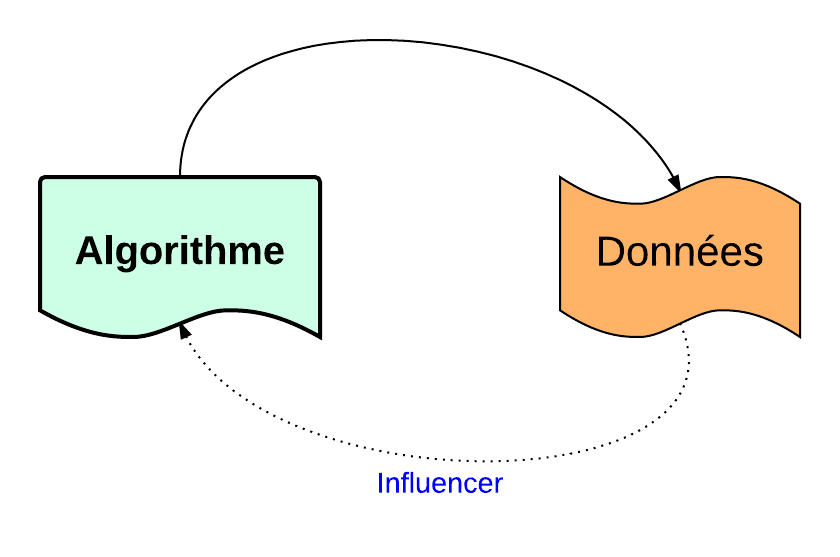
\includegraphics{sequentiel.png}}
\caption{Relation algorithme et données}\end{figure}
\begin{itemize}
\item {} 
Les donnees d'un algorithme doivent posséder la possibilité d'influencer les \textbf{instructions} d'un algorithme.

\end{itemize}


\subsection{Exécution séquentielle}
\label{structures1:execution-sequentielle}\begin{itemize}
\item {} 
Jusqu'à maintenant, nos programmes se limitaient au cas séquentiel. \emph{ie} (commandes ligne après ligne)

\end{itemize}

\begin{notice}{note}{Note:}
Les structure de \textbf{contrôle} permettent de changer ce comportement.
\end{notice}

Il existe trois structures de contrôle:
\begin{enumerate}
\item {} 
les \textbf{Branchement conditionnels}

\item {} 
Les itérations, (finie)

\item {} 
Les boucles \textbf{conditionnées}

\end{enumerate}


\bigskip\hrule{}\bigskip



\subsubsection{Branchement conditionnels}
\label{structures1:branchement-conditionnels}\begin{itemize}
\item {} 
Ces instructions permettent de \textbf{choisir} ou de \textbf{sauter} quelque \emph{instructions}, si certains \textbf{conditions} sont remplies. en utilisant le mot clé \textbf{if}.

\end{itemize}


\subsection{Exemple 1}
\label{structures1:exemple-1}
\begin{Verbatim}[commandchars=\\\{\},numbers=left,firstnumber=1,stepnumber=1]
\PYG{c+c1}{// codes/chap02/TesteurNote.java}

\PYG{k+kn}{import} \PYG{n+nn}{java.util.Scanner}\PYG{o}{;}


\PYG{k+kd}{public}  \PYG{k+kd}{class} \PYG{n+nc}{TesteurNote} \PYG{o}{\PYGZob{}}

    \PYG{k+kd}{public} \PYG{k+kd}{static} \PYG{k+kt}{void} \PYG{n+nf}{main}\PYG{o}{(}\PYG{n}{String}\PYG{o}{[}\PYG{o}{]} \PYG{n}{args}\PYG{o}{)} \PYG{o}{\PYGZob{}}

        \PYG{c+c1}{//variable qui va stocker la note}
        \PYG{k+kt}{float} \PYG{n}{note}\PYG{o}{;}

        \PYG{c+c1}{//Construire le Scanner}
        \PYG{n}{Scanner} \PYG{n}{input}\PYG{o}{=}\PYG{k}{new} \PYG{n}{Scanner}\PYG{o}{(}\PYG{n}{System}\PYG{o}{.}\PYG{n+na}{in}\PYG{o}{)}\PYG{o}{;}


        \PYG{c+c1}{//lecture d\PYGZsq{}une note}
        \PYG{n}{System}\PYG{o}{.}\PYG{n+na}{out}\PYG{o}{.}\PYG{n+na}{println}\PYG{o}{(}\PYG{l+s}{\PYGZdq{}Donner votre note: \PYGZdq{}}\PYG{o}{)}\PYG{o}{;}
        \PYG{n}{note}\PYG{o}{=}\PYG{n}{input}\PYG{o}{.}\PYG{n+na}{nextFloat}\PYG{o}{(}\PYG{o}{)}\PYG{o}{;}


        \PYG{c+c1}{//tester la valeur de la note pour décider du shcema a afficher}
        \PYG{k}{if}\PYG{o}{(}\PYG{n}{note}\PYG{o}{\PYGZgt{}}\PYG{o}{=}\PYG{l+m+mi}{10}\PYG{o}{)}
        \PYG{o}{\PYGZob{}}
            \PYG{n}{System}\PYG{o}{.}\PYG{n+na}{out}\PYG{o}{.}\PYG{n+na}{println}\PYG{o}{(}\PYG{l+s}{\PYGZdq{}votre note est \PYGZdq{}}\PYG{o}{+}\PYG{n}{note}\PYG{o}{)}\PYG{o}{;}
            \PYG{n}{System}\PYG{o}{.}\PYG{n+na}{out}\PYG{o}{.}\PYG{n+na}{println}\PYG{o}{(}\PYG{l+s}{\PYGZdq{}Vous avez réussi\PYGZdq{}}\PYG{o}{)}\PYG{o}{;}
        \PYG{o}{\PYGZcb{}}
        \PYG{k}{else}
        \PYG{o}{\PYGZob{}}
            \PYG{n}{System}\PYG{o}{.}\PYG{n+na}{out}\PYG{o}{.}\PYG{n+na}{println}\PYG{o}{(}\PYG{l+s}{\PYGZdq{}Votre note est \PYGZdq{}}\PYG{o}{+}\PYG{n}{note}\PYG{o}{)}\PYG{o}{;}
            \PYG{n}{System}\PYG{o}{.}\PYG{n+na}{out}\PYG{o}{.}\PYG{n+na}{println}\PYG{o}{(}\PYG{l+s}{\PYGZdq{}Désole, vous devez répéter le module\PYGZdq{}}\PYG{o}{)}\PYG{o}{;}
        \PYG{o}{\PYGZcb{}}

        \PYG{n}{System}\PYG{o}{.}\PYG{n+na}{out}\PYG{o}{.}\PYG{n+na}{println}\PYG{o}{(}\PYG{l+s}{\PYGZdq{}Au revoir\PYGZdq{}}\PYG{o}{)}\PYG{o}{;}

    \PYG{o}{\PYGZcb{}}
\PYG{o}{\PYGZcb{}}
\end{Verbatim}

ce code va \textbf{lire} la valeur de la note entrée par le clavier, et \textbf{selon} cette valeur, le programme va afficher un message \emph{convenable}.

\begin{notice}{note}{Note:}
On peut ajouter \textbf{autant} d'instructions dans le bloc \textbf{if} et \textbf{else}.
\end{notice}

\begin{Verbatim}[commandchars=\\\{\},numbers=left,firstnumber=1,stepnumber=1]
\PYG{c+c1}{// codes/chap02/TesteurNote2.java}

\PYG{k+kn}{import} \PYG{n+nn}{java.util.Scanner}\PYG{o}{;}


\PYG{k+kd}{public}  \PYG{k+kd}{class} \PYG{n+nc}{TesteurNote2}\PYG{o}{\PYGZob{}}

    \PYG{k+kd}{public} \PYG{k+kd}{static} \PYG{k+kt}{void} \PYG{n+nf}{main}\PYG{o}{(}\PYG{n}{String}\PYG{o}{[}\PYG{o}{]} \PYG{n}{args}\PYG{o}{)} \PYG{o}{\PYGZob{}}

        \PYG{c+c1}{//variable qui va stocker la note}
        \PYG{k+kt}{int} \PYG{n}{note}\PYG{o}{;}
        \PYG{c+c1}{//Construire le Scanner}
        \PYG{n}{Scanner} \PYG{n}{input}\PYG{o}{=}\PYG{k}{new} \PYG{n}{Scanner}\PYG{o}{(}\PYG{n}{System}\PYG{o}{.}\PYG{n+na}{in}\PYG{o}{)}\PYG{o}{;}


        \PYG{c+c1}{//lecture d\PYGZsq{}une note}
        \PYG{n}{System}\PYG{o}{.}\PYG{n+na}{out}\PYG{o}{.}\PYG{n+na}{println}\PYG{o}{(}\PYG{l+s}{\PYGZdq{}Donner votre note: \PYGZdq{}}\PYG{o}{)}\PYG{o}{;}
        \PYG{n}{note}\PYG{o}{=}\PYG{n}{input}\PYG{o}{.}\PYG{n+na}{nextInt}\PYG{o}{(}\PYG{o}{)}\PYG{o}{;}


        \PYG{c+c1}{//tester la valeur de la note pour décider du shcema a afficher}
        \PYG{k}{if}\PYG{o}{(}\PYG{n}{note}\PYG{o}{\PYGZgt{}}\PYG{o}{=}\PYG{l+m+mi}{10}\PYG{o}{)}
        \PYG{o}{\PYGZob{}}
            \PYG{n}{System}\PYG{o}{.}\PYG{n+na}{out}\PYG{o}{.}\PYG{n+na}{printf}\PYG{o}{(}\PYG{l+s}{\PYGZdq{}Votre note est \PYGZpc{}d\PYGZbs{}n\PYGZdq{}}\PYG{o}{,}\PYG{n}{note}\PYG{o}{)}\PYG{o}{;}
            \PYG{n}{System}\PYG{o}{.}\PYG{n+na}{out}\PYG{o}{.}\PYG{n+na}{println}\PYG{o}{(}\PYG{l+s}{\PYGZdq{}Vous avez réussi\PYGZdq{}}\PYG{o}{)}\PYG{o}{;}
        \PYG{o}{\PYGZcb{}}
        \PYG{k}{else}
        \PYG{o}{\PYGZob{}}
            \PYG{n}{System}\PYG{o}{.}\PYG{n+na}{out}\PYG{o}{.}\PYG{n+na}{printf}\PYG{o}{(}\PYG{l+s}{\PYGZdq{}Votre note est \PYGZpc{}d\PYGZbs{}n\PYGZdq{}}\PYG{o}{,}\PYG{n}{note}\PYG{o}{)}\PYG{o}{;}
            \PYG{n}{System}\PYG{o}{.}\PYG{n+na}{out}\PYG{o}{.}\PYG{n+na}{println}\PYG{o}{(}\PYG{l+s}{\PYGZdq{}Désole, vous devez répéter le module\PYGZdq{}}\PYG{o}{)}\PYG{o}{;}
        \PYG{o}{\PYGZcb{}}

        \PYG{n}{System}\PYG{o}{.}\PYG{n+na}{out}\PYG{o}{.}\PYG{n+na}{println}\PYG{o}{(}\PYG{l+s}{\PYGZdq{}Au revoir\PYGZdq{}}\PYG{o}{)}\PYG{o}{;}

    \PYG{o}{\PYGZcb{}}
\PYG{o}{\PYGZcb{}}
\end{Verbatim}

la syntaxe \textbf{générale} d'un branchement conditionnel est:

\begin{Verbatim}[commandchars=\\\{\}]
if(condition)
\PYGZob{}
    instructions
\PYGZcb{}
else if
\PYGZob{}
    instructions
\PYGZcb{}
else
\PYGZob{}
    instructions
\PYGZcb{}
\end{Verbatim}


\subsection{Choix imbriquées}
\label{structures1:choix-imbriquees}\begin{itemize}
\item {} 
Les instructions dans dans le blocs \textbf{if} et \textbf{else} peuvent contenir n'importe quel code java, et donc il peuvent contenir aussi une instruction \textbf{if} ce qui en résulte à des \textbf{choix imbriquées}.

\end{itemize}


\subsection{Exemple}
\label{structures1:exemple}
\begin{Verbatim}[commandchars=\\\{\},numbers=left,firstnumber=1,stepnumber=1]
\PYG{c+c1}{// codes/chap02/TesteurEgalite.java}

\PYG{k+kn}{import} \PYG{n+nn}{java.util.Scanner}\PYG{o}{;}


\PYG{k+kd}{class} \PYG{n+nc}{TesteurEgalite} \PYG{o}{\PYGZob{}}

    \PYG{k+kd}{public} \PYG{k+kd}{static} \PYG{k+kt}{void} \PYG{n+nf}{main}\PYG{o}{(}\PYG{n}{String}\PYG{o}{[}\PYG{o}{]} \PYG{n}{args}\PYG{o}{)} \PYG{o}{\PYGZob{}}

        \PYG{c+c1}{//declarer troix entiers}

        \PYG{k+kt}{int} \PYG{n}{d1}\PYG{o}{,}\PYG{n}{d2}\PYG{o}{,}\PYG{n}{d3}\PYG{o}{;}

        \PYG{c+c1}{//Declarer le Scanner}
        \PYG{n}{Scanner} \PYG{n}{input}\PYG{o}{=}\PYG{k}{new} \PYG{n}{Scanner}\PYG{o}{(}\PYG{n}{System}\PYG{o}{.}\PYG{n+na}{in}\PYG{o}{)}\PYG{o}{;}


        \PYG{c+c1}{//lecture des trois entiers}
        \PYG{n}{System}\PYG{o}{.}\PYG{n+na}{out}\PYG{o}{.}\PYG{n+na}{println}\PYG{o}{(}\PYG{l+s}{\PYGZdq{}Donner 3 entiers: \PYGZdq{}}\PYG{o}{)}\PYG{o}{;}
        \PYG{n}{d1}\PYG{o}{=}\PYG{n}{input}\PYG{o}{.}\PYG{n+na}{nextInt}\PYG{o}{(}\PYG{o}{)}\PYG{o}{;}
        \PYG{n}{d2}\PYG{o}{=}\PYG{n}{input}\PYG{o}{.}\PYG{n+na}{nextInt}\PYG{o}{(}\PYG{o}{)}\PYG{o}{;}
        \PYG{n}{d3}\PYG{o}{=}\PYG{n}{input}\PYG{o}{.}\PYG{n+na}{nextInt}\PYG{o}{(}\PYG{o}{)}\PYG{o}{;}


        \PYG{c+c1}{//tester l\PYGZsq{}égalité}
        \PYG{k}{if}\PYG{o}{(}\PYG{n}{d1}\PYG{o}{!}\PYG{o}{=}\PYG{n}{d2}\PYG{o}{)}
        \PYG{o}{\PYGZob{}}
            \PYG{n}{System}\PYG{o}{.}\PYG{n+na}{out}\PYG{o}{.}\PYG{n+na}{printf}\PYG{o}{(}\PYG{l+s}{\PYGZdq{}\PYGZpc{}d \PYGZsh{} \PYGZpc{}d\PYGZbs{}n\PYGZdq{}}\PYG{o}{,}\PYG{n}{d1}\PYG{o}{,}\PYG{n}{d2}\PYG{o}{)}\PYG{o}{;}
        \PYG{o}{\PYGZcb{}}
        \PYG{k}{else}
        \PYG{o}{\PYGZob{}}
            \PYG{k}{if}\PYG{o}{(}\PYG{n}{d2}\PYG{o}{!}\PYG{o}{=}\PYG{n}{d3}\PYG{o}{)}
            \PYG{o}{\PYGZob{}}
                \PYG{n}{System}\PYG{o}{.}\PYG{n+na}{out}\PYG{o}{.}\PYG{n+na}{printf}\PYG{o}{(}\PYG{l+s}{\PYGZdq{}\PYGZpc{}d \PYGZsh{} \PYGZpc{}d\PYGZbs{}n\PYGZdq{}}\PYG{o}{,}\PYG{n}{d2}\PYG{o}{,}\PYG{n}{d3}\PYG{o}{)}\PYG{o}{;}
            \PYG{o}{\PYGZcb{}}
            \PYG{k}{else}
            \PYG{o}{\PYGZob{}}
                \PYG{n}{System}\PYG{o}{.}\PYG{n+na}{out}\PYG{o}{.}\PYG{n+na}{println}\PYG{o}{(}\PYG{l+s}{\PYGZdq{}les trois sont egals\PYGZdq{}}\PYG{o}{)}\PYG{o}{;}
            \PYG{o}{\PYGZcb{}}
        \PYG{o}{\PYGZcb{}}

    \PYG{o}{\PYGZcb{}}
\PYG{o}{\PYGZcb{}}
\end{Verbatim}


\subsubsection{Opérateurs logiques}
\label{structures1:operateurs-logiques}\begin{itemize}
\item {} 
Une condition \textbf{simple} compare deux expressions, en utilisant les opérateurs de \textbf{comparaisons}

\end{itemize}


\subsection{Opérateurs de comparaison}
\label{structures1:operateurs-de-comparaison}

\begin{threeparttable}
\capstart\caption{Opérateurs de comparaison}

\begin{tabulary}{\linewidth}{|L|L|}
\hline
\textsf{\relax 
Opérateur
} & \textsf{\relax 
signification
}\\
\hline
\textless{}
 & 
inférieur à
\\
\hline
\textgreater{}
 & 
supérieur à
\\
\hline
\textless{}=
 & 
inférieur ou égal
\\
\hline
\textgreater{}=
 & 
supérieur ou égal
\\
\hline
==
 & 
égale à
\\
\hline
!=
 & 
différent de
\\
\hline\end{tabulary}

\end{threeparttable}



\bigskip\hrule{}\bigskip



\subsection{Opérateur logiques}
\label{structures1:operateur-logiques}
On peut relier des conditions \textbf{simples} par des opérateur \textbf{logiques}.

\textbf{L'opérateur logique ET(\&\&)}

qui est \textbf{Vrai*} si et seulement si tous les conditions simples sont \textbf{Vraies}.

\textbf{Exemple}:

\begin{Verbatim}[commandchars=\\\{\}]
(a\PYGZlt{}b) \PYGZam{}\PYGZam{} (b\PYGZlt{}c)
\end{Verbatim}

sera \textbf{Vrai} uniquement is \textbf{a\textless{}b} est \emph{vrai}, et \textbf{b\textless{}c} est \emph{vrai}.

\begin{Verbatim}[commandchars=\\\{\}]
\PYG{k}{if}\PYG{o}{(}\PYG{o}{(}\PYG{n}{note}\PYG{o}{\PYGZgt{}}\PYG{o}{=}\PYG{l+m+mi}{0}\PYG{o}{)} \PYG{o}{\PYGZam{}}\PYG{o}{\PYGZam{}} \PYG{o}{(}\PYG{n}{note}\PYG{o}{\PYGZlt{}}\PYG{o}{=}\PYG{l+m+mi}{20}\PYG{o}{)}\PYG{o}{)}
\PYG{o}{\PYGZob{}}
    \PYG{n}{System}\PYG{o}{.}\PYG{n+na}{out}\PYG{o}{.}\PYG{n+na}{println}\PYG{o}{(}\PYG{l+s}{\PYGZdq{}Note valide\PYGZdq{}}\PYG{o}{)}\PYG{o}{;}
\PYG{o}{\PYGZcb{}}
\PYG{k}{else}
\PYG{o}{\PYGZob{}}
    \PYG{n}{System}\PYG{o}{.}\PYG{n+na}{out}\PYG{o}{.}\PYG{n+na}{println}\PYG{o}{(}\PYG{l+s}{\PYGZdq{}Note non reconnue\PYGZdq{}}\PYG{o}{)}\PYG{o}{;}
\PYG{o}{\PYGZcb{}}
\end{Verbatim}


\bigskip\hrule{}\bigskip


\textbf{L'opérateur logique OU}

Est \textbf{Vrai*} si  \emph{seulement l'une*} des conditions simples est \textbf{Vraie}.

\textbf{Exemple}:

\begin{Verbatim}[commandchars=\\\{\}]
(m\PYGZgt{}0) \PYGZam{}\PYGZam{} (m\PYGZgt{}0)
\end{Verbatim}

sera \textbf{Vrai} l'une des valeurs \textbf{m} ou \textbf{n} est positive.

\begin{Verbatim}[commandchars=\\\{\}]
\PYG{k}{if}\PYG{o}{(}\PYG{o}{(}\PYG{n}{n}\PYG{o}{\PYGZgt{}}\PYG{l+m+mi}{0}\PYG{o}{)} \PYG{o}{\PYGZam{}}\PYG{o}{\PYGZam{}} \PYG{o}{(}\PYG{n}{m}\PYG{o}{\PYGZgt{}}\PYG{l+m+mi}{0}\PYG{o}{)}\PYG{o}{)}
\PYG{o}{\PYGZob{}}
    \PYG{n}{System}\PYG{o}{.}\PYG{n+na}{out}\PYG{o}{.}\PYG{n+na}{println}\PYG{o}{(}\PYG{l+s}{\PYGZdq{}L\PYGZsq{}une des valeurs est positive\PYGZdq{}}\PYG{o}{)}\PYG{o}{;}
\PYG{o}{\PYGZcb{}}
\PYG{k}{else}
\PYG{o}{\PYGZob{}}
    \PYG{n}{System}\PYG{o}{.}\PYG{n+na}{out}\PYG{o}{.}\PYG{n+na}{println}\PYG{o}{(}\PYG{l+s}{\PYGZdq{}les deux valeurs sont négatifs\PYGZdq{}}\PYG{o}{)}\PYG{o}{;}
\PYG{o}{\PYGZcb{}}
\end{Verbatim}


\begin{threeparttable}
\capstart\caption{Table logique}

\begin{tabulary}{\linewidth}{|L|L|L|L|}
\hline
\textsf{\relax 
P
} & \textsf{\relax 
Q
} & \textsf{\relax 
P et Q
} & \textsf{\relax 
P ou Q
}\\
\hline
Vrai
 & 
Vrai
 & 
Vrai
 & 
Vrai
\\
\hline
Vrai
 & 
Faux
 & 
Faux
 & 
Vrai
\\
\hline
Faux
 & 
Vrai
 & 
Faux
 & 
Vrai
\\
\hline
Faux
 & 
Faux
 & 
Faux
 & 
Faux
\\
\hline\end{tabulary}

\end{threeparttable}



\subsubsection{Erreurs classiques}
\label{structures1:erreurs-classiques}
Ici on regroupe quelque erreurs de débutants.


\subsection{test d'égalité}
\label{structures1:test-d-egalite}
\begin{Verbatim}[commandchars=\\\{\}]
\PYG{k}{if}\PYG{o}{(}\PYG{n}{a}\PYG{o}{=}\PYG{n}{b}\PYG{o}{)}  \PYG{c+c1}{// !!! ne sera pas accepté par le compilateur}
\end{Verbatim}


\subsection{if et ;}
\label{structures1:if-et}
\begin{Verbatim}[commandchars=\\\{\}]
\PYG{k}{if}\PYG{o}{(}\PYG{n}{a}\PYG{o}{=}\PYG{o}{=}\PYG{l+m+mi}{2}\PYG{o}{)}\PYG{o}{;} \PYG{o}{!}\PYG{o}{!}
    \PYG{n}{System}\PYG{o}{.}\PYG{n+na}{out}\PYG{o}{.}\PYG{n+na}{println}\PYG{o}{(}\PYG{l+s}{\PYGZdq{}a=\PYGZdq{}}\PYG{o}{+}\PYG{l+m+mi}{2}\PYG{o}{)}\PYG{o}{;}
\end{Verbatim}

Dans ce cas la message sera \textbf{toujours} affiché, quelque soit la valeur de \textbf{a}.


\subsection{else sans accolade}
\label{structures1:else-sans-accolade}
\begin{Verbatim}[commandchars=\\\{\}]
\PYG{k}{if}\PYG{o}{(} \PYG{n}{a}\PYG{o}{\PYGZlt{}}\PYG{n}{b}\PYG{o}{)}
    \PYG{n}{System}\PYG{o}{.}\PYG{n+na}{out}\PYG{o}{.}\PYG{n+na}{println}\PYG{o}{(}\PYG{l+s}{\PYGZdq{}a\PYGZlt{}b\PYGZdq{}}\PYG{o}{)}\PYG{o}{;}
    \PYG{n}{max}\PYG{o}{=}\PYG{n}{b}\PYG{o}{;}
\PYG{k}{else}  \PYG{c+c1}{//!!}

    \PYG{n}{System}\PYG{o}{.}\PYG{n+na}{out}\PYG{o}{.}\PYG{n+na}{println}\PYG{o}{(}\PYG{l+s}{\PYGZdq{}a\PYGZgt{}b\PYGZdq{}}\PYG{o}{)}\PYG{o}{;}
\end{Verbatim}

Donnera un message d'erreur.


\subsubsection{Exercices d'applications}
\label{structures1:exercices-d-applications}\begin{enumerate}
\item {} 
Ecrire un programme \textbf{MoyenneModule} qui demande une \textbf{note} à l'utilisateur,et vérifie s'ils sont valides. ie( \(\in [0,20]\)).

\item {} 
modifier \textbf{MoyenneModule} pour vérifier \textbf{deux} notes.

\item {} 
Calculer la moyenne des deux notes, puis informer l'utilisateur s'il a validé le module ou non.:

\begin{Verbatim}[commandchars=\\\{\}]
moyenne \PYGZgt{}=12     ===\PYGZgt{} validé
sinon            ===\PYGZgt{} non validé
\end{Verbatim}

\item {} 
Modifier le programme \textbf{TesteurEgalite.java} en ajoutant un test \emph{complexe} utilisant \textbf{Et}.

\item {} 
Écrivez un programme Java qui lit un nombre et indique s'il est positif, négatif ou s'il vaut zéro et s'il est pair ou impair.:

\begin{Verbatim}[commandchars=\\\{\}]
Entrez un nombre entier: 5
Le nombre est positif et impair

Entrez un nombre entier: \PYGZhy{}4
Le nombre est négatif et pair

Entrez un nombre entier: 0
Le nombre est zéro (et il est pair)
\end{Verbatim}

\end{enumerate}


\bigskip\hrule{}\bigskip



\subsubsection{Les boucles finies}
\label{structures1:les-boucles-finies}\begin{itemize}
\item {} 
Souvent dans un programme, on a besoin de \textbf{répéter} certains instructions pour aboutir à un résultat.

\end{itemize}

\textbf{Exemple:}

Afficher les carrés des 5 premiers entiers de \(\mathbb{N}\):

\begin{Verbatim}[commandchars=\\\{\}]
le carré de 0   est    0
le carré de 1   est    1
le carré de 2   est    4
le carré de 3   est    9
le carré de 4   est    16
\end{Verbatim}

On peut obtenir ce résultat en utilisant une boucle \textbf{for} comme suit.

\begin{Verbatim}[commandchars=\\\{\}]
\PYG{k}{for}\PYG{o}{(}\PYG{k+kt}{int} \PYG{n}{i}\PYG{o}{=}\PYG{l+m+mi}{0}\PYG{o}{;}\PYG{n}{i}\PYG{o}{\PYGZlt{}}\PYG{l+m+mi}{5}\PYG{o}{;}\PYG{n}{i}\PYG{o}{+}\PYG{o}{+}\PYG{o}{)}
    \PYG{n}{System}\PYG{o}{.}\PYG{n+na}{out}\PYG{o}{.}\PYG{n+na}{println}\PYG{o}{(}\PYG{l+s}{\PYGZdq{}le carré de \PYGZdq{}}\PYG{o}{+}\PYG{n}{i}\PYG{o}{+}\PYG{l+s}{\PYGZdq{} est \PYGZdq{}}\PYG{o}{+} \PYG{n}{i}\PYG{o}{*}\PYG{n}{i}\PYG{o}{)}\PYG{o}{;}
\end{Verbatim}

La boucle \textbf{for} contient trois parties qui sont
\begin{itemize}
\item {} 
initialisation
\begin{quote}

exécutée \emph{une seule} fois au début de la boucle.
\end{quote}

\item {} 
Test d'arrêt:
\begin{quote}

qui sera testé \textbf{avant} l'exécution de chaque tour de la boucle.
\end{quote}

\item {} 
Incrémentation:
\begin{quote}

Exécutée à la fin de chaque tour, elle permet de \textbf{changer} la valeur de \emph{compteur}.
\end{quote}

\end{itemize}

Donc la syntaxe générale d'une boucle for en \textbf{Java} est:

\begin{Verbatim}[commandchars=\\\{\}]
for(Initialisation; test d\PYGZsq{}arrêt; Incrémentation)
\PYGZob{}
             Bloc d\PYGZsq{}instructions;
\PYGZcb{}
\end{Verbatim}


\subsection{Exemple 2:}
\label{structures1:exemple-2}
Voici un deuxième exemple de la \textbf{table de multiplication} de \(7\).

\begin{Verbatim}[commandchars=\\\{\},numbers=left,firstnumber=1,stepnumber=1]
\PYG{c+c1}{// codes/chap02/TableMult7.java}


\PYG{k+kd}{class} \PYG{n+nc}{TableMult7}  \PYG{o}{\PYGZob{}}

    \PYG{k+kd}{public} \PYG{k+kd}{static} \PYG{k+kt}{void} \PYG{n+nf}{main}\PYG{o}{(}\PYG{n}{String}\PYG{o}{[}\PYG{o}{]} \PYG{n}{args}\PYG{o}{)} \PYG{o}{\PYGZob{}}

        \PYG{n}{System}\PYG{o}{.}\PYG{n+na}{out}\PYG{o}{.}\PYG{n+na}{println}\PYG{o}{(}\PYG{l+s}{\PYGZdq{}Table de multiplication de 7\PYGZdq{}}\PYG{o}{)}\PYG{o}{;}

        \PYG{k}{for} \PYG{o}{(}\PYG{k+kt}{int} \PYG{n}{i}\PYG{o}{=}\PYG{l+m+mi}{1}\PYG{o}{;}\PYG{n}{i}\PYG{o}{\PYGZlt{}}\PYG{o}{=}\PYG{l+m+mi}{7}\PYG{o}{;} \PYG{n}{i}\PYG{o}{+}\PYG{o}{+}\PYG{o}{)} \PYG{o}{\PYGZob{}}

            \PYG{n}{System}\PYG{o}{.}\PYG{n+na}{out}\PYG{o}{.}\PYG{n+na}{println}\PYG{o}{(}\PYG{l+s}{\PYGZdq{}5 *\PYGZdq{}}\PYG{o}{+}\PYG{n}{i}\PYG{o}{+}\PYG{l+s}{\PYGZdq{} = \PYGZdq{}}\PYG{o}{+}\PYG{l+m+mi}{5}\PYG{o}{*}\PYG{n}{i}\PYG{o}{)}\PYG{o}{;}
        \PYG{o}{\PYGZcb{}}
    \PYG{o}{\PYGZcb{}}
\PYG{o}{\PYGZcb{}}
\end{Verbatim}

Affichera

\begin{Verbatim}[commandchars=\\\{\}]
\PYG{l+m+mi}{5} \PYG{o}{*}\PYG{l+m+mi}{1} \PYG{o}{=} \PYG{l+m+mi}{5}
\PYG{l+m+mi}{5} \PYG{o}{*}\PYG{l+m+mi}{2} \PYG{o}{=} \PYG{l+m+mi}{10}
\PYG{l+m+mi}{5} \PYG{o}{*}\PYG{l+m+mi}{3} \PYG{o}{=} \PYG{l+m+mi}{15}
\PYG{l+m+mi}{5} \PYG{o}{*}\PYG{l+m+mi}{4} \PYG{o}{=} \PYG{l+m+mi}{20}
\PYG{l+m+mi}{5} \PYG{o}{*}\PYG{l+m+mi}{5} \PYG{o}{=} \PYG{l+m+mi}{25}
\PYG{l+m+mi}{5} \PYG{o}{*}\PYG{l+m+mi}{6} \PYG{o}{=} \PYG{l+m+mi}{30}
\PYG{l+m+mi}{5} \PYG{o}{*}\PYG{l+m+mi}{7} \PYG{o}{=} \PYG{l+m+mi}{35}
\end{Verbatim}

\begin{notice}{note}{Note:}
Le \textbf{bloc d'instruction} de for peut contenir n'importe quel \emph{code} java.
\end{notice}

Par exemple il peut contenir une instruction \textbf{if}

\textbf{Question}

Quel sera le résultat du programme suivant:

\begin{Verbatim}[commandchars=\\\{\}]
\PYG{k}{for}\PYG{o}{(}\PYG{k+kt}{int} \PYG{n}{i}\PYG{o}{=}\PYG{l+m+mi}{0}\PYG{o}{;}\PYG{n}{i}\PYG{o}{\PYGZlt{}}\PYG{l+m+mi}{5}\PYG{o}{;}\PYG{n}{i}\PYG{o}{+}\PYG{o}{+}\PYG{o}{)}
\PYG{o}{\PYGZob{}}
    \PYG{n}{System}\PYG{o}{.}\PYG{n+na}{out}\PYG{o}{.}\PYG{n+na}{print}\PYG{o}{(}\PYG{n}{i}\PYG{o}{)}\PYG{o}{;}

    \PYG{k}{if}\PYG{o}{(} \PYG{n}{i}\PYG{o}{\PYGZpc{}}\PYG{l+m+mi}{2}\PYG{o}{=}\PYG{o}{=}\PYG{l+m+mi}{0}\PYG{o}{)}
    \PYG{o}{\PYGZob{}}
        \PYG{n}{System}\PYG{o}{.}\PYG{n+na}{out}\PYG{o}{.}\PYG{n+na}{print}\PYG{o}{(}\PYG{l+s}{\PYGZdq{}p\PYGZdq{}}\PYG{o}{)}\PYG{o}{;}
    \PYG{o}{\PYGZcb{}}

    \PYG{n}{System}\PYG{o}{.}\PYG{n+na}{out}\PYG{o}{.}\PYG{n+na}{print}\PYG{o}{(}\PYG{l+s}{\PYGZdq{} \PYGZdq{}}\PYG{o}{)}\PYG{o}{;}
\PYG{o}{\PYGZcb{}}
\end{Verbatim}


\subsection{D'autre exemples}
\label{structures1:d-autre-exemples}
\textbf{Saut différent}

\begin{Verbatim}[commandchars=\\\{\}]
\PYG{k}{for}\PYG{o}{(}\PYG{k+kt}{int} \PYG{n}{p}\PYG{o}{=}\PYG{l+m+mi}{0}\PYG{o}{;}\PYG{n}{p}\PYG{o}{\PYGZlt{}}\PYG{l+m+mi}{10}\PYG{o}{;}\PYG{n}{p}\PYG{o}{=}\PYG{n}{p}\PYG{o}{+}\PYG{l+m+mi}{2}\PYG{o}{)}
    \PYG{n}{System}\PYG{o}{.}\PYG{n+na}{out}\PYG{o}{.}\PYG{n+na}{print}\PYG{o}{(}\PYG{n}{p}\PYG{o}{+}\PYG{l+s}{\PYGZdq{} \PYGZdq{}}\PYG{o}{)}\PYG{o}{;}
\end{Verbatim}

Affichera:

\begin{Verbatim}[commandchars=\\\{\}]
0  2  4  6  8
\end{Verbatim}

\begin{notice}{note}{Note:}
Dans cet exemple \textbf{p=p+2} pourrait être ecrit par \textbf{p+=2}
\end{notice}

\textbf{Décrémentation}

\begin{Verbatim}[commandchars=\\\{\}]
\PYG{k}{for}\PYG{o}{(}\PYG{k+kt}{int} \PYG{n}{k}\PYG{o}{=}\PYG{l+m+mi}{10}\PYG{o}{;}\PYG{n}{k}\PYG{o}{\PYGZgt{}}\PYG{l+m+mi}{5}\PYG{o}{;}\PYG{n}{k}\PYG{o}{\PYGZhy{}}\PYG{o}{\PYGZhy{}}\PYG{o}{)}
    \PYG{n}{System}\PYG{o}{.}\PYG{n+na}{out}\PYG{o}{.}\PYG{n+na}{println}\PYG{o}{(}\PYG{n}{k}\PYG{o}{+}\PYG{l+s}{\PYGZdq{} \PYGZdq{}}\PYG{o}{)}\PYG{o}{;}
\end{Verbatim}

Affichera:

\begin{Verbatim}[commandchars=\\\{\}]
10 9 8 7 6
\end{Verbatim}

\textbf{Exemple classique}

Dans ce simple programme on se propose de calculer la \textbf{moyenne} de \(10\) valeurs entrées par le clavier.

\begin{Verbatim}[commandchars=\\\{\},numbers=left,firstnumber=1,stepnumber=1]
\PYG{c+c1}{// codes/chap02/Moyenne10.java}


\PYG{k+kn}{import} \PYG{n+nn}{java.util.Scanner}\PYG{o}{;}


\PYG{k+kd}{class} \PYG{n+nc}{Moyenne10} \PYG{o}{\PYGZob{}}
    \PYG{k+kd}{public} \PYG{k+kd}{static} \PYG{k+kt}{void} \PYG{n+nf}{main}\PYG{o}{(}\PYG{n}{String}\PYG{o}{[}\PYG{o}{]} \PYG{n}{args}\PYG{o}{)} \PYG{o}{\PYGZob{}}

        \PYG{c+c1}{//declarer la variable de lecture}
        \PYG{k+kt}{double} \PYG{n}{note}\PYG{o}{;}

        \PYG{c+c1}{//declarer la somme et la moyenne}
        \PYG{k+kt}{double} \PYG{n}{somme}\PYG{o}{,}\PYG{n}{moyenne}\PYG{o}{;}

        \PYG{c+c1}{//construir un lecteur input avec le scanner}
        \PYG{n}{Scanner} \PYG{n}{clavier}\PYG{o}{=}\PYG{k}{new} \PYG{n}{Scanner}\PYG{o}{(}\PYG{n}{System}\PYG{o}{.}\PYG{n+na}{in}\PYG{o}{)}\PYG{o}{;}

        \PYG{c+c1}{//Toujours inialiser la somme à 0}
        \PYG{n}{somme}\PYG{o}{=}\PYG{l+m+mf}{0.0}\PYG{o}{;}

        \PYG{k}{for}\PYG{o}{(}\PYG{k+kt}{int} \PYG{n}{i}\PYG{o}{=}\PYG{l+m+mi}{1}\PYG{o}{;}\PYG{n}{i}\PYG{o}{\PYGZlt{}}\PYG{o}{=}\PYG{l+m+mi}{5}\PYG{o}{;}\PYG{n}{i}\PYG{o}{+}\PYG{o}{+}\PYG{o}{)}
        \PYG{o}{\PYGZob{}}
            \PYG{n}{System}\PYG{o}{.}\PYG{n+na}{out}\PYG{o}{.}\PYG{n+na}{print}\PYG{o}{(}\PYG{l+s}{\PYGZdq{}Enter la note \PYGZdq{}}\PYG{o}{+}\PYG{n}{i}\PYG{o}{+} \PYG{l+s}{\PYGZdq{}: \PYGZdq{}}\PYG{o}{)}\PYG{o}{;}
            \PYG{n}{note}\PYG{o}{=}\PYG{n}{clavier}\PYG{o}{.}\PYG{n+na}{nextDouble}\PYG{o}{(}\PYG{o}{)}\PYG{o}{;}

            \PYG{c+c1}{// Ajouter la note lue à la somme}
            \PYG{n}{somme}\PYG{o}{+}\PYG{o}{=}\PYG{n}{note}\PYG{o}{;}
        \PYG{o}{\PYGZcb{}}

        \PYG{c+c1}{//Calculer la moyenne(somme/5)}
        \PYG{n}{moyenne}\PYG{o}{=}\PYG{n}{somme}\PYG{o}{/}\PYG{l+m+mi}{5}\PYG{o}{;}

        \PYG{c+c1}{//Afficher la moyenne}

        \PYG{n}{System}\PYG{o}{.}\PYG{n+na}{out}\PYG{o}{.}\PYG{n+na}{println}\PYG{o}{(}\PYG{l+s}{\PYGZdq{}votre moyenne est \PYGZdq{}}\PYG{o}{+}\PYG{n}{moyenne}\PYG{o}{)}\PYG{o}{;}
    \PYG{o}{\PYGZcb{}}
\PYG{o}{\PYGZcb{}}
\end{Verbatim}

\textbf{boucle For imbriquées}

On peut introduit des boucle \textbf{for} à l'intérieur d'une boucle \textbf{for}.


\subsection{Exemple}
\label{structures1:id1}
Qeul sera le résultat du programme suivant:

\begin{Verbatim}[commandchars=\\\{\}]
\PYG{k}{for}\PYG{o}{(}\PYG{k+kt}{int} \PYG{n}{i}\PYG{o}{=}\PYG{l+m+mi}{0}\PYG{o}{;}\PYG{n}{i}\PYG{o}{\PYGZlt{}}\PYG{l+m+mi}{4}\PYG{o}{;}\PYG{n}{i}\PYG{o}{+}\PYG{o}{+}\PYG{o}{)}
    \PYG{o}{\PYGZob{}}
        \PYG{k}{for}\PYG{o}{(}\PYG{k+kt}{int} \PYG{n}{j}\PYG{o}{=}\PYG{l+m+mi}{0}\PYG{o}{;}\PYG{n}{j}\PYG{o}{\PYGZlt{}}\PYG{l+m+mi}{4}\PYG{o}{;}\PYG{n}{j}\PYG{o}{+}\PYG{o}{+}\PYG{o}{)}
        \PYG{o}{\PYGZob{}}
            \PYG{k}{if}\PYG{o}{(}\PYG{n}{i}\PYG{o}{=}\PYG{o}{=}\PYG{n}{j}\PYG{o}{)}
            \PYG{o}{\PYGZob{}}
                \PYG{n}{System}\PYG{o}{.}\PYG{n+na}{out}\PYG{o}{.}\PYG{n+na}{print}\PYG{o}{(}\PYG{l+s}{\PYGZdq{}*\PYGZdq{}}\PYG{o}{)}\PYG{o}{;}
            \PYG{o}{\PYGZcb{}}
            \PYG{k}{else}
            \PYG{o}{\PYGZob{}}
                \PYG{n}{System}\PYG{o}{.}\PYG{n+na}{out}\PYG{o}{.}\PYG{n+na}{print}\PYG{o}{(}\PYG{l+s}{\PYGZdq{}j\PYGZdq{}}\PYG{o}{)}\PYG{o}{;}
            \PYG{o}{\PYGZcb{}}
        \PYG{o}{\PYGZcb{}}

        \PYG{n}{System}\PYG{o}{.}\PYG{n+na}{out}\PYG{o}{.}\PYG{n+na}{println}\PYG{o}{(}\PYG{l+s}{\PYGZdq{} \PYGZdq{}}\PYG{o}{)}\PYG{o}{;}
    \PYG{o}{\PYGZcb{}}
\end{Verbatim}


\subsubsection{Exercices}
\label{structures1:exercices}\begin{enumerate}
\item {} 
(+) Ecrire un programme pour afficher les nombres \textbf{impairs} compris entre \(0\) et \(30\).

\item {} 
(++) Ecrire un programme pour calcule le produit entre deux entiers a et b positifs. en utilisant la formule suivante:

\end{enumerate}
\begin{gather}
\begin{split}ab=\underbrace{a+a+\ldots+a}_{b \; fois}\end{split}\notag
\end{gather}\begin{enumerate}
\setcounter{enumi}{2}
\item {} 
(+++)Ecrire un programme pour afficher la \textbf{table de multiplication}.

\end{enumerate}


\bigskip\hrule{}\bigskip



\subsubsection{Boucles conditionnelles}
\label{structures1:boucles-conditionnelles}
Selon le problème à résoudre. il arrive qu'on \textbf{ne connaisse} pas combien de fois la \emph{boucle*} devra être exécutée.

Dans ce cas, on utilise une \textbf{boucle conditionnelle}, ou boucle \textbf{while}, \textbf{do .. while}.


\subsection{Exemple:}
\label{structures1:id2}
Pour illustrer l'utilisation d'une boucle conditionnelle, on présentera un programme qui  as \textbf{besoin} que qu'une valeur \emph{nbNotes} soit \textbf{positive}.

\begin{Verbatim}[commandchars=\\\{\},numbers=left,firstnumber=1,stepnumber=1]
\PYG{c+cm}{/** Moyenne non controllée*/}

\PYG{k+kn}{import} \PYG{n+nn}{java.util.Scanner}\PYG{o}{;}



\PYG{k+kd}{public} \PYG{k+kd}{class} \PYG{n+nc}{Moyenne}\PYG{o}{\PYGZob{}}

    \PYG{k+kd}{public} \PYG{k+kd}{static} \PYG{k+kt}{void} \PYG{n+nf}{main}\PYG{o}{(}\PYG{n}{String}\PYG{o}{[}\PYG{o}{]} \PYG{n}{args}\PYG{o}{)} \PYG{o}{\PYGZob{}}

        \PYG{c+c1}{//lecture des nombres de notes}
        \PYG{n}{System}\PYG{o}{.}\PYG{n+na}{out}\PYG{o}{.}\PYG{n+na}{println}\PYG{o}{(}\PYG{l+s}{\PYGZdq{}Donner le nombre de notes: \PYGZdq{}}\PYG{o}{)}\PYG{o}{;}
        \PYG{n}{Scanner} \PYG{n}{clavier}\PYG{o}{=}\PYG{k}{new} \PYG{n}{Scanner}\PYG{o}{(}\PYG{n}{System}\PYG{o}{.}\PYG{n+na}{in}\PYG{o}{)}\PYG{o}{;}
        \PYG{k+kt}{int} \PYG{n}{nbNotes}\PYG{o}{=}\PYG{n}{clavier}\PYG{o}{.}\PYG{n+na}{nextInt}\PYG{o}{(}\PYG{o}{)}\PYG{o}{;}


        \PYG{k+kt}{float} \PYG{n}{somme}\PYG{o}{,}\PYG{n}{moyenne}\PYG{o}{;}

        \PYG{c+c1}{//vérifier si le nombre de notes est \PYGZgt{}0}

        \PYG{k}{if}\PYG{o}{(}\PYG{n}{nbNotes}\PYG{o}{\PYGZgt{}}\PYG{l+m+mi}{0}\PYG{o}{)}
        \PYG{o}{\PYGZob{}}

            \PYG{c+c1}{//executer une boule for pour calculer la moyenne}
            \PYG{n}{somme}\PYG{o}{=}\PYG{l+m+mi}{0}\PYG{o}{;}

            \PYG{k}{for}\PYG{o}{(}\PYG{k+kt}{int} \PYG{n}{i}\PYG{o}{=}\PYG{l+m+mi}{0}\PYG{o}{;}\PYG{n}{i}\PYG{o}{\PYGZlt{}}\PYG{n}{nbNotes}\PYG{o}{;}\PYG{n}{i}\PYG{o}{+}\PYG{o}{+}\PYG{o}{)}
            \PYG{o}{\PYGZob{}}
                \PYG{c+c1}{//lire la note i}
                \PYG{n}{System}\PYG{o}{.}\PYG{n+na}{out}\PYG{o}{.}\PYG{n+na}{println}\PYG{o}{(}\PYG{l+s}{\PYGZdq{}Donner une note: \PYGZdq{}}\PYG{o}{)}\PYG{o}{;}
                \PYG{n}{somme}\PYG{o}{+}\PYG{o}{=}\PYG{n}{clavier}\PYG{o}{.}\PYG{n+na}{nextFloat}\PYG{o}{(}\PYG{o}{)}\PYG{o}{;}
            \PYG{o}{\PYGZcb{}}

            \PYG{c+c1}{//calcul de la moyenne}
            \PYG{n}{moyenne}\PYG{o}{=}\PYG{n}{somme}\PYG{o}{/}\PYG{n}{nbNotes}\PYG{o}{;}

            \PYG{c+c1}{//Afficher la moyenne}
            \PYG{n}{System}\PYG{o}{.}\PYG{n+na}{out}\PYG{o}{.}\PYG{n+na}{println}\PYG{o}{(}\PYG{l+s}{\PYGZdq{}Votre moyenne est \PYGZdq{}}\PYG{o}{+}\PYG{n}{moyenne}\PYG{o}{)}\PYG{o}{;}
        \PYG{o}{\PYGZcb{}}
    \PYG{o}{\PYGZcb{}}
\PYG{o}{\PYGZcb{}}
\end{Verbatim}

Ici une valeur \textbf{négative} de l'utilisateur n'aura aucun sens. donc on se propose de \textbf{forcer} une condition sur cette valeur.
\begin{gather}
\begin{split}nbNotes>0\end{split}\notag
\end{gather}
Donc on va introduire une \textbf{boucle} qui va se répéter \textbf{tant que} cette valeur est \textbf{négative}.

\begin{Verbatim}[commandchars=\\\{\}]
\PYG{k}{do}
\PYG{o}{\PYGZob{}}
    \PYG{n}{System}\PYG{o}{.}\PYG{n+na}{out}\PYG{o}{.}\PYG{n+na}{println}\PYG{o}{(}\PYG{l+s}{\PYGZdq{}Entrer le nombre de notes:\PYGZdq{}}\PYG{o}{)}\PYG{o}{;}
    \PYG{n}{nbNotes}\PYG{o}{=}\PYG{n}{clavier}\PYG{o}{.}\PYG{n+na}{nextInt}\PYG{o}{(}\PYG{o}{)}\PYG{o}{;}
\PYG{o}{\PYGZcb{}}\PYG{k}{while}\PYG{o}{(}\PYG{n}{nbNotes}\PYG{o}{\PYGZlt{}}\PYG{o}{=}\PYG{l+m+mi}{0}\PYG{o}{)}
\end{Verbatim}
\begin{enumerate}
\item {} 
Modifier le programme \textbf{Moyenne1.java} pour refuser les valeurs négatifs de nbNotes

\end{enumerate}


\subsection{Syntaxe générale:}
\label{structures1:syntaxe-generale}
\begin{Verbatim}[commandchars=\\\{\}]
\PYG{k}{do}
\PYG{o}{\PYGZob{}}
    \PYG{n}{instructions}\PYG{o}{;}

\PYG{o}{\PYGZcb{}}\PYG{k}{while}\PYG{o}{(}\PYG{n}{condition}\PYG{o}{)}\PYG{o}{;}
\end{Verbatim}
\begin{itemize}
\item {} 
La condition peut utiliser des \emph{opérateurs logiques}.

\item {} 
la parenthèse autour de la condition sont \textbf{obligatoires}.

\end{itemize}

\begin{notice}{note}{Note:}
Les instructions à l'intérieur de \textbf{do while} seront toujours exécutées \textbf{au moins un fois}
\end{notice}


\subsection{Boucle while}
\label{structures1:boucle-while}
Dans certains conditions, on veut tester les conditions \textbf{a priori} avant d'enter dans le corps de la boucle. dans ce cas on utilise une deuxième forme de la boucle \textbf{while}.

\begin{Verbatim}[commandchars=\\\{\}]
\PYG{k}{while}\PYG{o}{(}\PYG{n}{condition}\PYG{o}{)}
\PYG{o}{\PYGZob{}}
    \PYG{n}{instructions}
\PYG{o}{\PYGZcb{}}
\end{Verbatim}
\begin{itemize}
\item {} 
Le principe est \textbf{similaire}, avec la seule différence que le test sera testé \textbf{avant} d'enter dans la boucle.

\item {} 
Donc les instructions de while peuvent \textbf{ne jamais} être exécutées.

\end{itemize}


\subsection{exemples}
\label{structures1:exemples}
\begin{Verbatim}[commandchars=\\\{\}]
\PYG{k+kt}{int} \PYG{n}{i}\PYG{o}{=}\PYG{l+m+mi}{100}\PYG{o}{;}
\PYG{k}{do}
\PYG{o}{\PYGZob{}}
    \PYG{n}{System}\PYG{o}{.}\PYG{n+na}{out}\PYG{o}{.}\PYG{n+na}{println}\PYG{o}{(}\PYG{l+s}{\PYGZdq{}Bonjour\PYGZdq{}}\PYG{o}{)}\PYG{o}{;}
\PYG{o}{\PYGZcb{}} \PYG{k}{while}\PYG{o}{(}\PYG{n}{i}\PYG{o}{\PYGZlt{}}\PYG{l+m+mi}{10}\PYG{o}{)}\PYG{o}{;}
\end{Verbatim}

Le programme affichera:

\begin{Verbatim}[commandchars=\\\{\}]
\PYG{n}{Bonjour}
\end{Verbatim}

par contre le programme suivant:

\begin{Verbatim}[commandchars=\\\{\}]
\PYG{k+kt}{int} \PYG{n}{i}\PYG{o}{=}\PYG{l+m+mi}{100}\PYG{o}{;}

\PYG{k}{while}\PYG{o}{(}\PYG{n}{i}\PYG{o}{\PYGZlt{}}\PYG{l+m+mi}{10}\PYG{o}{)}
\PYG{o}{\PYGZob{}}
    \PYG{n}{System}\PYG{o}{.}\PYG{n+na}{out}\PYG{o}{.}\PYG{n+na}{println}\PYG{o}{(}\PYG{l+s}{\PYGZdq{}Bonjour\PYGZdq{}}\PYG{o}{)}\PYG{o}{;}
\PYG{o}{\PYGZcb{}}
\end{Verbatim}

\textbf{N'affichera} rien car les instructions de la boucle ne sont jamais exécutées.


\bigskip\hrule{}\bigskip



\subsubsection{Exercice d'application}
\label{structures1:exercice-d-application}
Dans cet exercice on se propose, de développer le code d'un jeu \textbf{simple} de devinette d'un nombre entier. où la machine va choisir un nombre \emph{entier} dans \([0,10]\), et à l'utilisateur de deviner cette valeur.
\begin{enumerate}
\item {} 
Pour générer une valeur \textbf{aléatoire} entière on utilisera la \emph{classe} \textbf{Random} du package \emph{java.util}

\end{enumerate}

\begin{Verbatim}[commandchars=\\\{\}]
\PYG{k+kn}{import} \PYG{n+nn}{java.util.Random}\PYG{o}{;}

\PYG{c+c1}{//instancier un object Random}
\PYG{n}{Random} \PYG{n}{R}\PYG{o}{=}\PYG{k}{new} \PYG{n}{Random}\PYG{o}{(}\PYG{o}{)}\PYG{o}{;}

\PYG{c+c1}{//générer un nombre \PYGZlt{} n}
\PYG{k+kt}{int} \PYG{n}{a}\PYG{o}{=}\PYG{n}{R}\PYG{o}{.}\PYG{n+na}{nextInt}\PYG{o}{(}\PYG{n}{n}\PYG{o}{)}\PYG{o}{;}
\end{Verbatim}
\begin{enumerate}
\setcounter{enumi}{1}
\item {} 
Ecrire un programme \textbf{JeuDevinette.java} pour générer et \emph{afficher} 15 valeurs aléatoires inférieurs à \(10\).

\item {} 
Le but du jeu est de générer une valeur aléatoire \textless{}10, et demander à l'utilisateur de \textbf{deviner} ce nombre.
\begin{itemize}
\item {} 
Au cas d'égalité, le  jeu s'arrête.

\item {} 
Au cas \textless{}nombre, on informe l'utilisateur qu'il doit donner une valeur \textbf{inférieure}.

\item {} 
Au cas \textgreater{}nombre, on informe l'utilisetuer qu'il doit donner une valeur \textbf{supérieure}.

\end{itemize}

\item {} 
Modifier votre programme pour limiter le nombre d'essai à \textbf{Trois} essais maximum.

\end{enumerate}


\section{Tableaux}
\label{tableaux1::doc}\label{tableaux1:tableaux}

\subsection{Introduction}
\label{tableaux1:introduction}
La représentation des données se réduit aux types \textbf{élémentaires}
\begin{itemize}
\item {} 
int

\item {} 
double

\item {} 
boolean.

\end{itemize}

Ils permettent de représenter, dans des variables, des concepts \textbf{simples} du monde modélisé dans le programme :
\begin{itemize}
\item {} 
dimensions

\item {} 
sommes

\item {} 
tailles

\item {} 
expressions logiques

\item {} 
...

\end{itemize}

\begin{notice}{note}{Note:}
Cependant, de nombreuses données plus \textbf{sophistiquées} ne se réduisent pas à un objet informatique élémentaire.
\end{notice}

un langage de programmation évolué doit donc fournir le moyen de \textbf{composer} les types élémentaires pour construire des types plus complexes.


\subsubsection{Exemples de données structurées}
\label{tableaux1:exemples-de-donnees-structurees}

\begin{threeparttable}
\capstart\caption{Tableaux Age}

\begin{tabulary}{\linewidth}{|L|L|L|L|L|L|L|L|L|}
\hline

Age
 & 
34
 & 
12
 & 
32
 & 
25
 & 
18
 & 
19
 & 
26
 & 
34
\\
\hline\end{tabulary}

\end{threeparttable}


\textbf{structure complexe}


\begin{threeparttable}
\capstart\caption{Étudiants}

\begin{tabulary}{\linewidth}{|L|L|L|L|}
\hline

Etudiant
 & 
Age
 & 
CIN
 & 
Moyenne
\\
\hline
Eudiant1
 & 
24
 & 
3232
 & 
14.5
\\
\hline
Eudiant2
 & 
19
 & 
3451
 & 
16
\\
\hline
Eudiant3
 & 
25
 & 
6743
 & 
12.5
\\
\hline
Eudiant4
 & 
28
 & 
8752
 & 
13
\\
\hline\end{tabulary}

\end{threeparttable}



\subsubsection{Type de base et types évolues}
\label{tableaux1:type-de-base-et-types-evolues}
il y a une différence importante pour le langage \textbf{Java} entre les variables de base et les types de \textbf{bases} et les types \textbf{évolués}.
\begin{itemize}
\item {} 
Toute variable de type de base stocke directement une \textbf{valeur}.

\end{itemize}

\begin{Verbatim}[commandchars=\\\{\}]
\PYG{k+kt}{int} \PYG{n}{a}\PYG{o}{=}\PYG{l+m+mi}{3}\PYG{o}{;}              \PYG{c+c1}{// la variable a stock la valeur 3}
\end{Verbatim}
\begin{itemize}
\item {} 
Toute variable de type évolué, comme les \textbf{tableaux} ou les \textbf{chaînes de caractères} (String), stocke une référence(adresse) vers une valeur :

\end{itemize}

\begin{Verbatim}[commandchars=\\\{\}]
\PYG{n}{String} \PYG{n}{ch}\PYG{o}{=}\PYG{l+s}{\PYGZdq{}Message\PYGZdq{}}\PYG{o}{;}        \PYG{c+c1}{// la variable ch contient une référence vers message}
\end{Verbatim}

\begin{notice}{note}{Note:}
Toute variable de type évolué stocke une \textbf{référence} vers une valeur
\end{notice}

\begin{notice}{warning}{Warning:}
ceci a une très grande incidence sur la sémantique des opérateurs \textbf{=} et \textbf{==} en Java !
\end{notice}

voici un simple exemple illustratif:

\begin{Verbatim}[commandchars=\\\{\},numbers=left,firstnumber=1,stepnumber=1]
\PYG{c+c1}{// codes/chap04/SipleVsEvolue.java}



\PYG{k+kd}{public} \PYG{k+kd}{class} \PYG{n+nc}{SimpleVsEvolue}
\PYG{o}{\PYGZob{}}

    \PYG{k+kd}{public} \PYG{k+kd}{static} \PYG{k+kt}{void} \PYG{n+nf}{main}\PYG{o}{(}\PYG{n}{String}\PYG{o}{[}\PYG{o}{]} \PYG{n}{args}\PYG{o}{)} \PYG{o}{\PYGZob{}}

        \PYG{c+c1}{//illustrer qu\PYGZsq{}une variable elementaire stock une valeur}

        \PYG{k+kt}{int} \PYG{n}{a}\PYG{o}{=}\PYG{l+m+mi}{3}\PYG{o}{;}  \PYG{c+c1}{//variable a stock la valeur 3}
        \PYG{k+kt}{int} \PYG{n}{b}\PYG{o}{=}\PYG{n}{a}\PYG{o}{;}  \PYG{c+c1}{//b recoie la valeur de a qui est 3}
        \PYG{n}{b}\PYG{o}{=}\PYG{l+m+mi}{4}\PYG{o}{;}      \PYG{c+c1}{// ceci modifie le contenu de b et pas celle de a}

        \PYG{n}{System}\PYG{o}{.}\PYG{n+na}{out}\PYG{o}{.}\PYG{n+na}{printf}\PYG{o}{(}\PYG{l+s}{\PYGZdq{}a=\PYGZpc{}d\PYGZbs{}tb=\PYGZpc{}d\PYGZbs{}n\PYGZdq{}}\PYG{o}{,}\PYG{n}{a}\PYG{o}{,}\PYG{n}{b}\PYG{o}{)}\PYG{o}{;}

        \PYG{c+c1}{//Appliquer la même traitement pour des String}
        \PYG{n}{String} \PYG{n}{ch1}\PYG{o}{=}\PYG{l+s}{\PYGZdq{}message\PYGZdq{}}\PYG{o}{;}
        \PYG{n}{String} \PYG{n}{ch2}\PYG{o}{=}\PYG{n}{ch1}\PYG{o}{;}       \PYG{c+c1}{//ch1 et ch2 se refère à la meme valeur}
    \PYG{o}{\PYGZcb{}}
\PYG{o}{\PYGZcb{}}
\end{Verbatim}


\subsubsection{Exemple Simple}
\label{tableaux1:exemple-simple}
On se propose d'écrire un programme qui demande la \emph{saisi} d'un nombre d'employée, puis leur \textbf{nombre d'article vendu}, puis affiche leur \textbf{moyenne} mais surtout \textbf{l'écart} de chaque employée à la moyenne.


\bigskip\hrule{}\bigskip



\subsection{Déclaration}
\label{tableaux1:declaration}
Il y as deux syntaxes générales pour déclarer un tableau en \textbf{java}:

\begin{Verbatim}[commandchars=\\\{\}]
TypeElement [] nomTableau
TypeElement  nomTableau[]
\end{Verbatim}

\textbf{Exemples}

\begin{Verbatim}[commandchars=\\\{\}]
\PYG{k+kt}{float}\PYG{o}{[}\PYG{o}{]} \PYG{n}{poids}\PYG{o}{;}
\PYG{k+kt}{int}   \PYG{n}{IP}\PYG{o}{[}\PYG{o}{]}\PYG{o}{;}
\end{Verbatim}


\subsubsection{Initialisation}
\label{tableaux1:initialisation}
Si on connaît les \textbf{valeurs} du tableau lors de la déclaration on peut utiliser.

\begin{Verbatim}[commandchars=\\\{\}]
\PYG{k+kt}{int} \PYG{n}{De}\PYG{o}{[}\PYG{l+m+mi}{6}\PYG{o}{]}\PYG{o}{=}\PYG{o}{\PYGZob{}}\PYG{l+m+mi}{1}\PYG{o}{,}\PYG{l+m+mi}{2}\PYG{o}{,}\PYG{l+m+mi}{3}\PYG{o}{,}\PYG{l+m+mi}{4}\PYG{o}{,}\PYG{l+m+mi}{5}\PYG{o}{,}\PYG{l+m+mi}{6}\PYG{o}{\PYGZcb{}}\PYG{o}{;}

\PYG{k+kt}{int} \PYG{n}{Reponses}\PYG{o}{[}\PYG{o}{]}\PYG{o}{=}\PYG{o}{\PYGZob{}}\PYG{l+m+mi}{1}\PYG{o}{,}\PYG{l+m+mi}{0}\PYG{o}{,}\PYG{l+m+mi}{0}\PYG{o}{,}\PYG{l+m+mi}{0}\PYG{o}{,}\PYG{l+m+mi}{1}\PYG{o}{\PYGZcb{}} \PYG{c+c1}{//java peut calculer la taille d\PYGZsq{}après les éléments}
\end{Verbatim}

\begin{notice}{note}{Note:}
La variable De contient une adresse : \textbf{l’emplacement} du tableau en mémoire !
\end{notice}

Si on connaît pas les valeurs du tableaux lors de la \textbf{déclaration}.

\begin{Verbatim}[commandchars=\\\{\}]
\PYG{k+kt}{float} \PYG{n}{notes}\PYG{o}{[}\PYG{o}{]}\PYG{o}{;}  \PYG{c+c1}{//déclaration}
\PYG{n}{notes}\PYG{o}{=}\PYG{k}{new} \PYG{k+kt}{float}\PYG{o}{[}\PYG{n}{taille}\PYG{o}{]}  \PYG{c+c1}{// réserver la taille au tableau}
\end{Verbatim}


\subsubsection{Valeur par défaut}
\label{tableaux1:valeur-par-defaut}
Si les valeurs du tableaux ne sont pas fournis, le tableau reçoit une valeur par \textbf{défaut}


\begin{threeparttable}
\capstart\caption{Valeur par Defaut}

\begin{tabulary}{\linewidth}{|L|L|}
\hline
\textsf{\relax 
type
} & \textsf{\relax 
valeur
}\\
\hline
int
 & 
0
\\
\hline
float
 & 
0.0
\\
\hline
bloolean
 & 
false
\\
\hline
autre
 & 
null
\\
\hline\end{tabulary}

\end{threeparttable}



\subsubsection{Accès aux élements}
\label{tableaux1:acces-aux-elements}
L'accès aux éléments se fait par l'opérateur \textbf{{[}{]}}.

\begin{Verbatim}[commandchars=\\\{\}]
\PYG{k+kt}{int} \PYG{n}{D}\PYG{o}{[}\PYG{o}{]}\PYG{o}{=}\PYG{o}{\PYGZob{}}\PYG{l+m+mi}{1}\PYG{o}{,}\PYG{l+m+mi}{2}\PYG{o}{,}\PYG{l+m+mi}{3}\PYG{o}{,}\PYG{l+m+mi}{4}\PYG{o}{,}\PYG{l+m+mi}{5}\PYG{o}{,}\PYG{l+m+mi}{6}\PYG{o}{\PYGZcb{}}\PYG{o}{;}

\PYG{c+c1}{//Afficher la deuxième composante de D}
\PYG{n}{System}\PYG{o}{.}\PYG{n+na}{out}\PYG{o}{.}\PYG{n+na}{println}\PYG{o}{(}\PYG{n}{D}\PYG{o}{[}\PYG{l+m+mi}{1}\PYG{o}{]}\PYG{o}{)}\PYG{o}{;}

\PYG{c+c1}{//Affichera le dernier élément}
\PYG{n}{System}\PYG{o}{.}\PYG{n+na}{out}\PYG{o}{.}\PYG{n+na}{println}\PYG{o}{(}\PYG{n}{D}\PYG{o}{[}\PYG{l+m+mi}{5}\PYG{o}{]}\PYG{o}{)}\PYG{o}{;}
\end{Verbatim}

\begin{notice}{warning}{Warning:}
Pour un tableau de taille \textbf{T} les indices varient de \textbf{0} à \textbf{T-1}.
\end{notice}


\subsection{Traitement}
\label{tableaux1:traitement}

\subsubsection{Affichage d'un tableau}
\label{tableaux1:affichage-d-un-tableau}
Dans cette partie on présentera des méthodes pour afficher un Tableau
\begin{itemize}
\item {} 
Le code suivant:

\end{itemize}

\begin{Verbatim}[commandchars=\\\{\}]
\PYG{k+kt}{double}\PYG{o}{[}\PYG{o}{]} \PYG{n}{T}\PYG{o}{=}\PYG{o}{\PYGZob{}}\PYG{l+m+mf}{1.2}\PYG{o}{,}\PYG{l+m+mf}{3.4}\PYG{o}{,}\PYG{o}{\PYGZhy{}}\PYG{l+m+mi}{5}\PYG{o}{,}\PYG{l+m+mi}{9}\PYG{o}{\PYGZcb{}}\PYG{o}{;}

\PYG{n}{System}\PYG{o}{.}\PYG{n+na}{out}\PYG{o}{.}\PYG{n+na}{println}\PYG{o}{(}\PYG{n}{T}\PYG{o}{)}\PYG{o}{;}
\end{Verbatim}

Affichera la \textbf{référence} du tableau \textbf{T}, donc une adresse.
\begin{itemize}
\item {} 
Donc si on veut afficher les éléments du tableau, il faudra appeler une boucle \textbf{for}.

\end{itemize}


\subsubsection{Accès aux éléments}
\label{tableaux1:id1}
Très souvent on voudrais accéder aux éléments d'un tableau, en effectuant une itérations sur ce tableau.
\begin{itemize}
\item {} 
Il existe au moins trois façons pour d'itérer sur un tableau.

\end{itemize}
\begin{enumerate}
\item {} 
Avec une \emph{itération} classique \textbf{for}.

\end{enumerate}

\begin{Verbatim}[commandchars=\\\{\}]
\PYG{k}{for}\PYG{o}{(}\PYG{k+kt}{int} \PYG{n}{i}\PYG{o}{=}\PYG{l+m+mi}{0}\PYG{o}{;}\PYG{n}{i}\PYG{o}{\PYGZlt{}}\PYG{n}{T}\PYG{o}{.}\PYG{n+na}{length}\PYG{o}{;}\PYG{n}{i}\PYG{o}{+}\PYG{o}{+}\PYG{o}{)}
\end{Verbatim}

\textbf{Exemple}

\begin{Verbatim}[commandchars=\\\{\}]
\PYG{k}{for}\PYG{o}{(}\PYG{k+kt}{int} \PYG{n}{i}\PYG{o}{=}\PYG{l+m+mi}{0}\PYG{o}{;}\PYG{n}{i}\PYG{o}{\PYGZlt{}}\PYG{n}{T}\PYG{o}{.}\PYG{n+na}{length}\PYG{o}{;} \PYG{n}{i}\PYG{o}{+}\PYG{o}{+}\PYG{o}{)}
    \PYG{n}{System}\PYG{o}{.}\PYG{n+na}{out}\PYG{o}{.}\PYG{n+na}{println}\PYG{o}{(}\PYG{n}{T}\PYG{o}{[}\PYG{n}{i}\PYG{o}{]}\PYG{o}{)}\PYG{o}{;}      \PYG{c+c1}{//Afficher les éléments du tableau}
\end{Verbatim}


\bigskip\hrule{}\bigskip

\begin{enumerate}
\setcounter{enumi}{1}
\item {} 
Avec des itérations sur un \textbf{ensemble de valeurs}.

\end{enumerate}

\begin{Verbatim}[commandchars=\\\{\}]
\PYG{k}{for}\PYG{o}{(}\PYG{n}{Type} \PYG{n+nl}{element:} \PYG{n}{Tableau}\PYG{o}{)}

    \PYG{c+c1}{//instructions}
\end{Verbatim}

\textbf{Exemple}

\begin{Verbatim}[commandchars=\\\{\}]
\PYG{c+c1}{//Déclarer le tableau}
\PYG{k+kt}{double} \PYG{n}{T}\PYG{o}{[}\PYG{o}{]}\PYG{o}{=}\PYG{o}{\PYGZob{}}\PYG{l+m+mf}{3.4}\PYG{o}{,}\PYG{o}{\PYGZhy{}}\PYG{l+m+mi}{2}\PYG{o}{,}\PYG{l+m+mi}{23}\PYG{o}{,}\PYG{l+m+mf}{12.3}\PYG{o}{\PYGZcb{}}\PYG{o}{;}

\PYG{c+c1}{//boucle sur le tableau}
\PYG{k}{for}\PYG{o}{(}\PYG{k+kt}{double} \PYG{n+nl}{val:} \PYG{n}{T}\PYG{o}{)}
    \PYG{n}{System}\PYG{o}{.}\PYG{n+na}{out}\PYG{o}{.}\PYG{n+na}{println}\PYG{o}{(}\PYG{n}{T}\PYG{o}{)}\PYG{o}{;}
\end{Verbatim}

\begin{notice}{note}{Note:}
Cette forme de boucle (\textbf{for}) contient certains \textbf{limites} comparée à la version classique.
\end{notice}
\begin{itemize}
\item {} 
Ne permet pas \textbf{modifier} le contenu du tableau.

\item {} 
Ne permet d’itérer que sur un \textbf{seul tableau} à la fois.

\item {} 
Ne permet l’accès qu’à un \textbf{seul élément} : on ne peut pas par exemple comparer un élément du tableau et son suivant.

\item {} 
Itere d'un pas en \textbf{avant} seulement.

\end{itemize}


\bigskip\hrule{}\bigskip

\begin{enumerate}
\setcounter{enumi}{2}
\item {} 
En utilisant les \textbf{itérateurs}, sera traité dans les derniers chapitres

\end{enumerate}


\subsubsection{Copie d'un Tableau}
\label{tableaux1:copie-d-un-tableau}
Qule sera le résultat du programme suivant:

\begin{Verbatim}[commandchars=\\\{\},numbers=left,firstnumber=1,stepnumber=1]
\PYG{c+c1}{//codes/chap04/TestCopie.java}


\PYG{k+kd}{public} \PYG{k+kd}{class} \PYG{n+nc}{TestCopie}
\PYG{o}{\PYGZob{}}
    \PYG{k+kd}{public} \PYG{k+kd}{static} \PYG{k+kt}{void} \PYG{n+nf}{main}\PYG{o}{(}\PYG{n}{String}\PYG{o}{[}\PYG{o}{]} \PYG{n}{args}\PYG{o}{)} \PYG{o}{\PYGZob{}}

        \PYG{c+c1}{//Déclarer un tableau A}
        \PYG{k+kt}{int} \PYG{n}{t1}\PYG{o}{[}\PYG{o}{]}\PYG{o}{=}\PYG{o}{\PYGZob{}}\PYG{l+m+mi}{1}\PYG{o}{,}\PYG{l+m+mi}{2}\PYG{o}{,}\PYG{l+m+mi}{3}\PYG{o}{,}\PYG{l+m+mi}{4}\PYG{o}{,}\PYG{l+m+mi}{5}\PYG{o}{,}\PYG{l+m+mi}{6}\PYG{o}{\PYGZcb{}}\PYG{o}{;}
        \PYG{k+kt}{int} \PYG{n}{t2}\PYG{o}{[}\PYG{o}{]}\PYG{o}{;}

        \PYG{c+c1}{//copie de t1 dans t2}
        \PYG{n}{t2}\PYG{o}{=}\PYG{n}{t1}\PYG{o}{;}

        \PYG{c+c1}{//modification d\PYGZsq{}un élement de t1}
        \PYG{n}{t1}\PYG{o}{[}\PYG{l+m+mi}{0}\PYG{o}{]}\PYG{o}{=}\PYG{l+m+mi}{4}\PYG{o}{;}

        \PYG{c+c1}{//Afficher t2}
        \PYG{k}{for} \PYG{o}{(}\PYG{k+kt}{int} \PYG{n}{elem} \PYG{o}{:} \PYG{n}{t1}\PYG{o}{)} \PYG{o}{\PYGZob{}}
            \PYG{n}{System}\PYG{o}{.}\PYG{n+na}{out}\PYG{o}{.}\PYG{n+na}{println}\PYG{o}{(}\PYG{n}{elem}\PYG{o}{)}\PYG{o}{;}
        \PYG{o}{\PYGZcb{}}
    \PYG{o}{\PYGZcb{}}
\PYG{o}{\PYGZcb{}}
\end{Verbatim}

\begin{notice}{warning}{Warning:}
l'instruction t1=t2 n'affecte pas les éléments de t1 dans t2, mais juste affecte \textbf{l'adresse} de t1 à t2.
\end{notice}

donc pour copier le tableaux \(T_1\) dans \(T_2\), on écrit:

\begin{Verbatim}[commandchars=\\\{\}]
\PYG{k}{for}\PYG{o}{(}\PYG{k+kt}{int} \PYG{n}{i}\PYG{o}{=}\PYG{l+m+mi}{0}\PYG{o}{;}\PYG{n}{i}\PYG{o}{\PYGZlt{}}\PYG{n}{t1}\PYG{o}{.}\PYG{n+na}{length}\PYG{o}{;}\PYG{n}{i}\PYG{o}{+}\PYG{o}{+}\PYG{o}{)}
\PYG{o}{\PYGZob{}}
    \PYG{n}{t2}\PYG{o}{[}\PYG{n}{i}\PYG{o}{]}\PYG{o}{=}\PYG{n}{t1}\PYG{o}{[}\PYG{n}{i}\PYG{o}{]}\PYG{o}{;}
\PYG{o}{\PYGZcb{}}
\end{Verbatim}


\subsubsection{Comparaison entre deux tableaux}
\label{tableaux1:comparaison-entre-deux-tableaux}
idem à l'opérateur \textbf{=} l'opérateur \textbf{==} va comparer les adresses des tableaux et non leurs valeurs.

\begin{Verbatim}[commandchars=\\\{\}]
\PYG{n}{t1}\PYG{o}{=}\PYG{o}{=}\PYG{n}{t2}\PYG{o}{;}        \PYG{c+c1}{// sera vrai, si t1 et t2 ont la même adresse.}
\end{Verbatim}

\begin{notice}{note}{Note:}
Donc pour \textbf{comparer} les valeurs d'un tableau, il faudra utiliser une boucle \textbf{for} voir (exercices)
\end{notice}


\subsection{Exercices}
\label{tableaux1:exercices}\begin{enumerate}
\item {} 
Un coureur enregistre la distance qu'il a parcouru chaque jours dans son entraînement. il a obtenu les valeurs suivants:

\end{enumerate}


\begin{threeparttable}
\capstart\caption{Distances}

\begin{tabulary}{\linewidth}{|L|L|L|L|L|L|L|L|L|L|L|L|}
\hline

12
 & 
8
 & 
11
 & 
13
 & 
12
 & 
9
 & 
10
 & 
8
 & 
11
 & 
12
 & 
10
 & 
12
\\
\hline\end{tabulary}

\end{threeparttable}


écrire un programme java \textbf{Distances.java} pour enregistrer ces distances, et puis:
\begin{itemize}
\item {} 
affiche les résultats

\item {} 
calcule somme totale qu'il a parcouru.

\item {} 
estime une moyenne par jour.

\end{itemize}
\begin{enumerate}
\setcounter{enumi}{1}
\item {} 
Ajouter le calcul de l'élément \textbf{minimal} et \textbf{maximal} dans le tableau.

\end{enumerate}
\begin{description}
\item[{3.(+++) Ecrire un programme qui}] \leavevmode\begin{itemize}
\item {} 
demande à l'utilisateur d'entrer une valeur positive \(n_1\), qui représente la taille de votre tableau.

\item {} 
Déclare un tableau de taille \(n_1\).

\item {} 
Remplir le tableau par des valeurs \textbf{aléatoires} entre 1 et 6; (voir chapitre précédant)

\item {} 
Afficher le nombre de \textbf{3} que vous avez obtenu.

\end{itemize}

\end{description}


\section{Fonctions et Méthodes}
\label{fonctions:fonctions-et-methodes}\label{fonctions::doc}\begin{itemize}
\item {} 
Dans cette partie du cours, on va présenter les notions qui vont nous aider à \textbf{organiser} notre code en le modélisant à l'aide de nos \emph{propres} fonctions.

\item {} 
Les \textbf{fonctions} font partie des aspects de traitement au même titre que les expressions et structures de contrôle.

\end{itemize}

\begin{notice}{note}{Note:}
Jusqu’à maintenant les programmes qu'on a développés sont constitués d'une séquence \textbf{linéaire} d'instructions, sans \textbf{organisation} globale, et sans \textbf{partage} des taches \emph{répétées}.
\end{notice}


\subsection{Notion de Réutilisabilité}
\label{fonctions:notion-de-reutilisabilite}
Supposons que le contrôle d'une entrée:

\begin{Verbatim}[commandchars=\\\{\}]
\PYG{k}{do}
\PYG{o}{\PYGZob{}}
    \PYG{n}{System}\PYG{o}{.}\PYG{n+na}{out}\PYG{o}{.}\PYG{n+na}{println}\PYG{o}{(}\PYG{l+s}{\PYGZdq{}Donner une note: \PYGZdq{}}\PYG{o}{)}\PYG{o}{;}
    \PYG{n}{note}\PYG{o}{=}\PYG{n}{clavier}\PYG{o}{.}\PYG{n+na}{nextDouble}\PYG{o}{(}\PYG{o}{)}\PYG{o}{;}
\PYG{o}{\PYGZcb{}}\PYG{k}{while}\PYG{o}{(}\PYG{o}{(}\PYG{n}{note}\PYG{o}{\PYGZlt{}}\PYG{l+m+mi}{0}\PYG{o}{)} \PYG{o}{\textbar{}}\PYG{o}{\textbar{}} \PYG{o}{(}\PYG{n}{note}\PYG{o}{\PYGZgt{}}\PYG{l+m+mi}{20}\PYG{o}{)}\PYG{o}{)}\PYG{o}{;}
\end{Verbatim}

doit être \textbf{répétée} dans plusieurs parties du programme.

\begin{notice}{warning}{Warning:}
\textbf{bonne pratique} : Ne jamais dupliquer un code en programmant, donc éviter le fameux \emph{copier/coller}.
\end{notice}

Généralement si vous voulez copier un code, c'est un indice que vous avez besoin d'une \textbf{fonction}.


\subsubsection{Mauvaise répitition:}
\label{fonctions:mauvaise-repitition}
\begin{Verbatim}[commandchars=\\\{\},numbers=left,firstnumber=1,stepnumber=1]
\PYG{c+c1}{//codes/chap05/Score1.java}

\PYG{k+kn}{import} \PYG{n+nn}{java.util.Scanner}\PYG{o}{;}



\PYG{k+kd}{class} \PYG{n+nc}{Score1} \PYG{o}{\PYGZob{}}

    \PYG{k+kd}{public} \PYG{k+kd}{static} \PYG{k+kt}{void} \PYG{n+nf}{main}\PYG{o}{(}\PYG{n}{String}\PYG{o}{[}\PYG{o}{]} \PYG{n}{args}\PYG{o}{)} \PYG{o}{\PYGZob{}}

        \PYG{c+cm}{/** Programme pour lire le nombre de points et le temps deux deux joueurs puis afficher leur score}
\PYG{c+cm}{        */}

        \PYG{c+c1}{//Clavier D\PYGZsq{}entrée}
        \PYG{n}{Scanner} \PYG{n}{clavier}\PYG{o}{=}\PYG{k}{new} \PYG{n}{Scanner}\PYG{o}{(}\PYG{n}{System}\PYG{o}{.}\PYG{n+na}{in}\PYG{o}{)}\PYG{o}{;}

        \PYG{c+c1}{//Lire le nombre de points du premier joueur}
        \PYG{k+kt}{int} \PYG{n}{nbPoints}\PYG{o}{;}

        \PYG{k}{do}
        \PYG{o}{\PYGZob{}}
            \PYG{n}{System}\PYG{o}{.}\PYG{n+na}{out}\PYG{o}{.}\PYG{n+na}{println}\PYG{o}{(}\PYG{l+s}{\PYGZdq{}Donner votre nombre de points (1\PYGZhy{}\PYGZhy{}100): \PYGZdq{}}\PYG{o}{)}\PYG{o}{;}
            \PYG{n}{nbPoints}\PYG{o}{=}\PYG{n}{clavier}\PYG{o}{.}\PYG{n+na}{nextInt}\PYG{o}{(}\PYG{o}{)}\PYG{o}{;}
        \PYG{o}{\PYGZcb{}}\PYG{k}{while}\PYG{o}{(} \PYG{n}{nbPoints}\PYG{o}{\PYGZlt{}}\PYG{l+m+mi}{0} \PYG{o}{\textbar{}}\PYG{o}{\textbar{}}  \PYG{n}{nbPoints}\PYG{o}{\PYGZgt{}}\PYG{l+m+mi}{100} \PYG{o}{)}\PYG{o}{;}


        \PYG{c+c1}{//lire le temps du joueur}
        \PYG{k+kt}{double} \PYG{n}{temps}\PYG{o}{;}
        \PYG{k}{do}
        \PYG{o}{\PYGZob{}}
            \PYG{n}{System}\PYG{o}{.}\PYG{n+na}{out}\PYG{o}{.}\PYG{n+na}{println}\PYG{o}{(}\PYG{l+s}{\PYGZdq{}donner votre temps (1\PYGZhy{}\PYGZhy{}60)\PYGZdq{}}\PYG{o}{)}\PYG{o}{;}
            \PYG{n}{temps}\PYG{o}{=}\PYG{n}{clavier}\PYG{o}{.}\PYG{n+na}{nextDouble}\PYG{o}{(}\PYG{o}{)}\PYG{o}{;}
        \PYG{o}{\PYGZcb{}}\PYG{k}{while}\PYG{o}{(}\PYG{n}{temps}\PYG{o}{\PYGZlt{}}\PYG{l+m+mi}{0} \PYG{o}{\textbar{}}\PYG{o}{\textbar{}} \PYG{n}{temps}\PYG{o}{\PYGZgt{}}\PYG{l+m+mi}{60}\PYG{o}{)}\PYG{o}{;}

        \PYG{c+c1}{//Calculer le score du premier joueur}
        \PYG{k+kt}{int} \PYG{n}{score1}\PYG{o}{=}\PYG{o}{(}\PYG{k+kt}{int}\PYG{o}{)}\PYG{o}{(}\PYG{l+m+mi}{40}\PYG{o}{*}\PYG{n}{nbPoints}\PYG{o}{/}\PYG{n}{temps}\PYG{o}{)}\PYG{o}{;}


        \PYG{c+c1}{//Score du deuxième joueur}
        \PYG{k}{do}
        \PYG{o}{\PYGZob{}}
            \PYG{n}{System}\PYG{o}{.}\PYG{n+na}{out}\PYG{o}{.}\PYG{n+na}{println}\PYG{o}{(}\PYG{l+s}{\PYGZdq{}Donner votre nombre de points (1\PYGZhy{}\PYGZhy{}100): \PYGZdq{}}\PYG{o}{)}\PYG{o}{;}
            \PYG{n}{nbPoints}\PYG{o}{=}\PYG{n}{clavier}\PYG{o}{.}\PYG{n+na}{nextInt}\PYG{o}{(}\PYG{o}{)}\PYG{o}{;}
        \PYG{o}{\PYGZcb{}}\PYG{k}{while}\PYG{o}{(} \PYG{n}{nbPoints}\PYG{o}{\PYGZlt{}}\PYG{l+m+mi}{0} \PYG{o}{\textbar{}}\PYG{o}{\textbar{}}  \PYG{n}{nbPoints}\PYG{o}{\PYGZgt{}}\PYG{l+m+mi}{100} \PYG{o}{)}\PYG{o}{;}


        \PYG{c+c1}{//lire le temps du joueur}
        \PYG{k}{do}
        \PYG{o}{\PYGZob{}}
            \PYG{n}{System}\PYG{o}{.}\PYG{n+na}{out}\PYG{o}{.}\PYG{n+na}{println}\PYG{o}{(}\PYG{l+s}{\PYGZdq{}donner votre temps (1\PYGZhy{}\PYGZhy{}60)\PYGZdq{}}\PYG{o}{)}\PYG{o}{;}
            \PYG{n}{temps}\PYG{o}{=}\PYG{n}{clavier}\PYG{o}{.}\PYG{n+na}{nextDouble}\PYG{o}{(}\PYG{o}{)}\PYG{o}{;}
        \PYG{o}{\PYGZcb{}}\PYG{k}{while}\PYG{o}{(}\PYG{n}{temps}\PYG{o}{\PYGZlt{}}\PYG{l+m+mi}{0} \PYG{o}{\textbar{}}\PYG{o}{\textbar{}} \PYG{n}{temps}\PYG{o}{\PYGZgt{}}\PYG{l+m+mi}{60}\PYG{o}{)}\PYG{o}{;}

        \PYG{c+c1}{//Calculer le score du premier joueur}
        \PYG{k+kt}{int} \PYG{n}{score2}\PYG{o}{=}\PYG{o}{(}\PYG{k+kt}{int}\PYG{o}{)}\PYG{o}{(}\PYG{l+m+mi}{40}\PYG{o}{*}\PYG{n}{nbPoints}\PYG{o}{/}\PYG{n}{temps}\PYG{o}{)}\PYG{o}{;}

        \PYG{c+c1}{//Afficher les scores}
        \PYG{n}{System}\PYG{o}{.}\PYG{n+na}{out}\PYG{o}{.}\PYG{n+na}{printf}\PYG{o}{(}\PYG{l+s}{\PYGZdq{}score joueur 1 est \PYGZpc{}d\PYGZbs{}n\PYGZdq{}}\PYG{o}{,}\PYG{n}{score1}\PYG{o}{)}\PYG{o}{;}
        \PYG{n}{System}\PYG{o}{.}\PYG{n+na}{out}\PYG{o}{.}\PYG{n+na}{printf}\PYG{o}{(}\PYG{l+s}{\PYGZdq{}score joueur 2 est \PYGZpc{}d\PYGZbs{}n\PYGZdq{}}\PYG{o}{,}\PYG{n}{score2}\PYG{o}{)}\PYG{o}{;}
    \PYG{o}{\PYGZcb{}}
\PYG{o}{\PYGZcb{}}
\end{Verbatim}

Malgré que ce code est lent , il ne contient que des taches simples. a titre d'exemple la \textbf{saisie} des données. et le calcul du \textbf{score}.

\begin{Verbatim}[commandchars=\\\{\}]
\PYG{k+kd}{static} \PYG{k+kt}{int} \PYG{n+nf}{saisieEtCalcul}\PYG{o}{(}\PYG{o}{)}
\PYG{o}{\PYGZob{}}
    \PYG{k+kt}{int} \PYG{n}{nbPoints}\PYG{o}{;}

    \PYG{k}{do}
    \PYG{o}{\PYGZob{}}
        \PYG{n}{System}\PYG{o}{.}\PYG{n+na}{out}\PYG{o}{.}\PYG{n+na}{println}\PYG{o}{(}\PYG{l+s}{\PYGZdq{}Donner votre nombre de points (1\PYGZhy{}\PYGZhy{}100): \PYGZdq{}}\PYG{o}{)}\PYG{o}{;}
        \PYG{n}{nbPoints}\PYG{o}{=}\PYG{n}{clavier}\PYG{o}{.}\PYG{n+na}{nextInt}\PYG{o}{(}\PYG{o}{)}\PYG{o}{;}
    \PYG{o}{\PYGZcb{}}\PYG{k}{while}\PYG{o}{(} \PYG{n}{nbPoints}\PYG{o}{\PYGZlt{}}\PYG{l+m+mi}{0} \PYG{o}{\textbar{}}\PYG{o}{\textbar{}}  \PYG{n}{nbPoints}\PYG{o}{\PYGZgt{}}\PYG{l+m+mi}{100} \PYG{o}{)}\PYG{o}{;}


    \PYG{c+c1}{//lire le temps du joueur}
    \PYG{k+kt}{double} \PYG{n}{temps}\PYG{o}{;}
    \PYG{k}{do}
    \PYG{o}{\PYGZob{}}
        \PYG{n}{System}\PYG{o}{.}\PYG{n+na}{out}\PYG{o}{.}\PYG{n+na}{println}\PYG{o}{(}\PYG{l+s}{\PYGZdq{}donner votre temps (1\PYGZhy{}\PYGZhy{}60)\PYGZdq{}}\PYG{o}{)}\PYG{o}{;}
        \PYG{n}{temps}\PYG{o}{=}\PYG{n}{clavier}\PYG{o}{.}\PYG{n+na}{nextDouble}\PYG{o}{(}\PYG{o}{)}\PYG{o}{;}
    \PYG{o}{\PYGZcb{}}\PYG{k}{while}\PYG{o}{(}\PYG{n}{temps}\PYG{o}{\PYGZlt{}}\PYG{l+m+mi}{0} \PYG{o}{\textbar{}}\PYG{o}{\textbar{}} \PYG{n}{temps}\PYG{o}{\PYGZgt{}}\PYG{l+m+mi}{60}\PYG{o}{)}\PYG{o}{;}

    \PYG{c+c1}{//Calculer le score du premier joueur}
    \PYG{k+kt}{int} \PYG{n}{score}\PYG{o}{=}\PYG{o}{(}\PYG{k+kt}{int}\PYG{o}{)}\PYG{o}{(}\PYG{l+m+mi}{40}\PYG{o}{*}\PYG{n}{nbPoints}\PYG{o}{/}\PYG{n}{temps}\PYG{o}{)}\PYG{o}{;}

    \PYG{c+c1}{//retourner la valeur de calcul}
    \PYG{k}{return} \PYG{n}{score}\PYG{o}{;}

\PYG{o}{\PYGZcb{}}
\end{Verbatim}

Aussi on pourra faire la même chose pour le calcul du score.

\begin{Verbatim}[commandchars=\\\{\}]
\PYG{k+kd}{static} \PYG{k+kt}{int} \PYG{n+nf}{calculerScore}\PYG{o}{(}\PYG{k+kt}{int}  \PYG{n}{nbPoints}\PYG{o}{,}\PYG{k+kt}{double} \PYG{n}{temps}\PYG{o}{)}
\PYG{o}{\PYGZob{}}
    \PYG{k}{if}\PYG{o}{(}\PYG{n}{temps}\PYG{o}{!}\PYG{o}{=}\PYG{l+m+mi}{0}\PYG{o}{)}
    \PYG{o}{\PYGZob{}}
       \PYG{k}{return} \PYG{o}{(}\PYG{k+kt}{int}\PYG{o}{)}\PYG{o}{(}\PYG{l+m+mi}{40}\PYG{o}{*}\PYG{n}{nbPoints}\PYG{o}{/}\PYG{n}{temps}\PYG{o}{)}
    \PYG{o}{\PYGZcb{}}
    \PYG{k}{else}
    \PYG{o}{\PYGZob{}}
        \PYG{k}{return} \PYG{l+m+mi}{0}\PYG{o}{;}
    \PYG{o}{\PYGZcb{}}
\PYG{o}{\PYGZcb{}}
\end{Verbatim}


\bigskip\hrule{}\bigskip



\subsection{Fonctions}
\label{fonctions:fonctions}
Une \textbf{fonction}: est une portion du programme réutilisable, ou importante en soi.

et qui est caractérisée par:
\begin{itemize}
\item {} 
\textbf{corps} : la portion du programme a réusitilisée, ou mettre en évidence.

\item {} 
\textbf{Nom}   : par lequel on va désigner cette fonction.

\item {} 
\textbf{arguments} : ensemble de variables extérieurs à la fonction, dont le \emph{corps} dépend pour fonctionner.

\item {} 
\textbf{Valeur de retour} : Ce que la fonction renvoie au reste du programme.

\end{itemize}

\begin{notice}{note}{Note:}
L'utilisation d'une fonction dans autre partie du programme, se nomme \textbf{appel} de la fonction.
\end{notice}


\subsubsection{Trois facettes d'une fonction}
\label{fonctions:trois-facettes-d-une-fonction}
Dans un programme on peut rencontrer une fonction sous l'une des formes suivantes:
\begin{figure}[htbp]
\centering
\capstart

\scalebox{0.500000}{\includegraphics{diagram_fonctions.png}}
\caption{Différents utilisation d'une fonction}\end{figure}
\begin{itemize}
\item {} 
Utilisation(appel):

\end{itemize}

Action d'utiliser une fonction, en l'appelant dans un programme.

\begin{center}exemple
\end{center}
\begin{Verbatim}[commandchars=\\\{\}]
\PYG{c+c1}{//fonction sans valeur de retour ni arguments}
\PYG{n}{saisieEtCalcul}\PYG{o}{(}\PYG{o}{)}\PYG{o}{;}

\PYG{c+c1}{//fonction sans valeur de retour, mais avec arguments}
\PYG{n}{triTableau}\PYG{o}{(}\PYG{n}{T}\PYG{o}{)}\PYG{o}{;}

\PYG{c+c1}{//fonction avec une valeur de retour, et arguments}
\PYG{k+kt}{char} \PYG{n}{c}\PYG{o}{=}\PYG{n}{getClass}\PYG{o}{(}\PYG{n}{ip}\PYG{o}{)}\PYG{o}{;}
\end{Verbatim}
\begin{itemize}
\item {} 
Création(définition):

\end{itemize}

Action de définir, et \textbf{implémenter} (préciser le corps) d'une fonction.

\begin{Verbatim}[commandchars=\\\{\}]
\PYG{k+kt}{double} \PYG{n+nf}{min}\PYG{o}{(}\PYG{k+kt}{double} \PYG{n}{a}\PYG{o}{,}\PYG{k+kt}{double} \PYG{n}{b}\PYG{o}{)}
\PYG{o}{\PYGZob{}}
    \PYG{c+c1}{//calculer le min;}
    \PYG{k+kt}{double} \PYG{n}{resultat}\PYG{o}{=}\PYG{o}{(}\PYG{n}{a}\PYG{o}{\PYGZlt{}}\PYG{n}{b}\PYG{o}{)}\PYG{o}{?}\PYG{n+nl}{a:}\PYG{n}{b}\PYG{o}{;}

    \PYG{c+c1}{//retourner la valeur calculée}
    \PYG{k}{return} \PYG{n}{resultat}\PYG{o}{;}
\PYG{o}{\PYGZcb{}}
\end{Verbatim}
\begin{itemize}
\item {} 
Résumé (Contrat):

\end{itemize}

Action de préciser juste la \textbf{définition} ou le \emph{prototype} d'une fonction, sans préciser sans corps.

\begin{Verbatim}[commandchars=\\\{\}]
\PYG{c+c1}{//prototype des fonctions précédentes}
\PYG{k+kt}{void} \PYG{n+nf}{saisieEtCalcul}\PYG{o}{(}\PYG{o}{)}\PYG{o}{;}

\PYG{c+c1}{//fonction pour trier un tableau}
\PYG{k+kt}{void} \PYG{n+nf}{triTableau}\PYG{o}{(}\PYG{k+kt}{double} \PYG{o}{[}\PYG{o}{]}\PYG{o}{)}\PYG{o}{;}

\PYG{c+c1}{//fonction pour obtenir une classe d\PYGZsq{}un ip}
\PYG{k+kt}{char} \PYG{n+nf}{getClass}\PYG{o}{(}\PYG{n}{Ip} \PYG{o}{)}\PYG{o}{;}
\end{Verbatim}


\subsection{Passage d'arguments}
\label{fonctions:passage-d-arguments}
Considérons la situation suivante:

\begin{Verbatim}[commandchars=\\\{\}]
\PYG{k+kd}{static} \PYG{k+kt}{void} \PYG{n+nf}{methode}\PYG{o}{(}\PYG{n}{Type} \PYG{n}{v}\PYG{o}{)}
\PYG{o}{\PYGZob{}}
   \PYG{c+c1}{// la fonction contient un traitement qui modifie v}
\PYG{o}{\PYGZcb{}}

\PYG{c+c1}{//Ailleurs dans le programme principal}
\PYG{n}{Type} \PYG{n}{v1}\PYG{o}{=}\PYG{o}{.}\PYG{o}{.}\PYG{o}{.}\PYG{o}{.}\PYG{o}{;}

\PYG{c+c1}{//appel de la fonction}
\PYG{n}{methode}\PYG{o}{(}\PYG{n}{v1}\PYG{o}{)}\PYG{o}{;}

\PYG{c+c1}{//Question qui se pose: est ce que v1 sera modifiée.}
\end{Verbatim}

En \textbf{Programmation} de façon générale, on dira que:
\begin{itemize}
\item {} 
L'argument v est \textbf{passé par valeur}, si \emph{méthode}  ne peut pas modifier v1, car v est une \textbf{copie} de v1.

\item {} 
L'argument v est \textbf{passé par référence}, si \emph{méthode} peut modifier v1.

\end{itemize}

\begin{notice}{warning}{Warning:}
En Java, il n'existe que le passage par \textbf{valeur}, (ie) une méthode travaille toujours sur une \textbf{copie} de la valeur qui lui est passée en paramètre.
\end{notice}

donc si \textbf{Type} est un type élémentaire. la valeur de \textbf{v1} ne sera pas changée.

\begin{center}Exemple
\end{center}
\begin{Verbatim}[commandchars=\\\{\},numbers=left,firstnumber=1,stepnumber=1]
\PYG{c+c1}{//codes/chap05/Passage1.java}


\PYG{k+kd}{class} \PYG{n+nc}{Passage1} \PYG{o}{\PYGZob{}}

    \PYG{k+kd}{public} \PYG{k+kd}{static} \PYG{k+kt}{void} \PYG{n+nf}{main}\PYG{o}{(}\PYG{n}{String}\PYG{o}{[}\PYG{o}{]} \PYG{n}{args}\PYG{o}{)} \PYG{o}{\PYGZob{}}

        \PYG{k+kt}{double} \PYG{n}{a}\PYG{o}{=}\PYG{l+m+mf}{3.2}\PYG{o}{;}

        \PYG{n}{System}\PYG{o}{.}\PYG{n+na}{out}\PYG{o}{.}\PYG{n+na}{println}\PYG{o}{(}\PYG{l+s}{\PYGZdq{}valeur de a est =\PYGZdq{}}\PYG{o}{+}\PYG{n}{a}\PYG{o}{)}\PYG{o}{;}

        \PYG{c+c1}{//essai de modifier le contenu de a par une méthode simple}
        \PYG{n}{augmenter}\PYG{o}{(}\PYG{n}{a}\PYG{o}{)}\PYG{o}{;}

        \PYG{c+c1}{//Afficher a après}
        \PYG{n}{System}\PYG{o}{.}\PYG{n+na}{out}\PYG{o}{.}\PYG{n+na}{println}\PYG{o}{(}\PYG{l+s}{\PYGZdq{}valeur de a est =\PYGZdq{}}\PYG{o}{+}\PYG{n}{a}\PYG{o}{)}\PYG{o}{;}

    \PYG{o}{\PYGZcb{}}

    \PYG{k+kd}{static} \PYG{k+kt}{void} \PYG{n+nf}{augmenter}\PYG{o}{(}\PYG{k+kt}{double} \PYG{n}{a}\PYG{o}{)}
    \PYG{o}{\PYGZob{}}
        \PYG{c+c1}{//méthode qui va essayer d\PYGZsq{}augmenter la valeur de a}
        \PYG{n}{a}\PYG{o}{+}\PYG{o}{=}\PYG{l+m+mi}{3}\PYG{o}{;}

        \PYG{n}{System}\PYG{o}{.}\PYG{n+na}{out}\PYG{o}{.}\PYG{n+na}{println}\PYG{o}{(}\PYG{l+s}{\PYGZdq{}Dans la fonction: valeur de a est =\PYGZdq{}}\PYG{o}{+}\PYG{n}{a}\PYG{o}{)}\PYG{o}{;}

    \PYG{o}{\PYGZcb{}}
\PYG{o}{\PYGZcb{}}
\end{Verbatim}


\subsubsection{Passage par valeur: Type évolué.}
\label{fonctions:passage-par-valeur-type-evolue}\begin{itemize}
\item {} 
Pour le type évolué, c'est toujours un passage par valeur, mais cette fois ci c'est la \textbf{référence} qui est copiée.

\end{itemize}

et donc

\begin{notice}{note}{Note:}
Toute modification faite sur l'objet référence via \textbf{la copie} est visible via \textbf{l'origine}.
\end{notice}

\begin{center}Exemple
\end{center}
\begin{Verbatim}[commandchars=\\\{\},numbers=left,firstnumber=1,stepnumber=1]
\PYG{c+c1}{//codes/chap05/Passage2.java}


\PYG{k+kd}{class} \PYG{n+nc}{Passage2} \PYG{o}{\PYGZob{}}

    \PYG{k+kd}{public} \PYG{k+kd}{static} \PYG{k+kt}{void} \PYG{n+nf}{main}\PYG{o}{(}\PYG{n}{String}\PYG{o}{[}\PYG{o}{]} \PYG{n}{args}\PYG{o}{)} \PYG{o}{\PYGZob{}}

        \PYG{c+c1}{//Declérer un référence sur un tableau}
        \PYG{k+kt}{int}\PYG{o}{[}\PYG{o}{]} \PYG{n}{T}\PYG{o}{=}\PYG{o}{\PYGZob{}}\PYG{l+m+mi}{1}\PYG{o}{,}\PYG{l+m+mi}{2}\PYG{o}{\PYGZcb{}}\PYG{o}{;}

        \PYG{c+c1}{//Afficher le tableau par une fonction}
        \PYG{n}{System}\PYG{o}{.}\PYG{n+na}{out}\PYG{o}{.}\PYG{n+na}{printf}\PYG{o}{(}\PYG{l+s}{\PYGZdq{}Tab = \PYGZpc{}d\PYGZbs{}t\PYGZpc{}d\PYGZbs{}n\PYGZdq{}}\PYG{o}{,}\PYG{n}{T}\PYG{o}{[}\PYG{l+m+mi}{0}\PYG{o}{]}\PYG{o}{,}\PYG{n}{T}\PYG{o}{[}\PYG{l+m+mi}{1}\PYG{o}{]}\PYG{o}{)}\PYG{o}{;}


        \PYG{c+c1}{//Modifier les valeur du tableau par une fonction}
        \PYG{n}{augmenter}\PYG{o}{(}\PYG{n}{T}\PYG{o}{)}\PYG{o}{;}

        \PYG{n}{System}\PYG{o}{.}\PYG{n+na}{out}\PYG{o}{.}\PYG{n+na}{println}\PYG{o}{(}\PYG{l+s}{\PYGZdq{}nouvelle valeurs de T\PYGZdq{}}\PYG{o}{)}\PYG{o}{;}
        \PYG{c+c1}{//Afficher le résultats}
        \PYG{n}{System}\PYG{o}{.}\PYG{n+na}{out}\PYG{o}{.}\PYG{n+na}{printf}\PYG{o}{(}\PYG{l+s}{\PYGZdq{}Tab = \PYGZpc{}d\PYGZbs{}t\PYGZpc{}d\PYGZbs{}n\PYGZdq{}}\PYG{o}{,}\PYG{n}{T}\PYG{o}{[}\PYG{l+m+mi}{0}\PYG{o}{]}\PYG{o}{,}\PYG{n}{T}\PYG{o}{[}\PYG{l+m+mi}{1}\PYG{o}{]}\PYG{o}{)}\PYG{o}{;}

    \PYG{o}{\PYGZcb{}}

    \PYG{k+kd}{static} \PYG{k+kt}{void} \PYG{n+nf}{augmenter}\PYG{o}{(}\PYG{k+kt}{int} \PYG{o}{[}\PYG{o}{]} \PYG{n}{Tab}\PYG{o}{)}
    \PYG{o}{\PYGZob{}}
        \PYG{c+c1}{//fonction pour changer le contenu d\PYGZsq{}un tableau}
        \PYG{k}{for}\PYG{o}{(}\PYG{k+kt}{int} \PYG{n}{i}\PYG{o}{=}\PYG{l+m+mi}{0}\PYG{o}{;}\PYG{n}{i}\PYG{o}{\PYGZlt{}}\PYG{n}{Tab}\PYG{o}{.}\PYG{n+na}{length}\PYG{o}{;}\PYG{n}{i}\PYG{o}{+}\PYG{o}{+}\PYG{o}{)}
        \PYG{o}{\PYGZob{}}
            \PYG{n}{Tab}\PYG{o}{[}\PYG{n}{i}\PYG{o}{]}\PYG{o}{+}\PYG{o}{=}\PYG{l+m+mi}{1}\PYG{o}{;}
        \PYG{o}{\PYGZcb{}}
    \PYG{o}{\PYGZcb{}}
\PYG{o}{\PYGZcb{}}
\end{Verbatim}


\paragraph{L'instruction return}
\label{fonctions:l-instruction-return}
L'instruction \textbf{return} est utilisée pour indiquer la valeur de retour d'une fonction.

\begin{notice}{note}{Note:}
L'instruction \emph{return} \textbf{termine} l'exécution d'une fonction.
\end{notice}

Supposons qu'on as défini la fonction suivante.

\begin{Verbatim}[commandchars=\\\{\}]
\PYG{k+kt}{boolean} \PYG{n+nf}{afficherInfo}\PYG{o}{(}\PYG{k+kt}{int} \PYG{n}{n}\PYG{o}{)}
\PYG{o}{\PYGZob{}}
     \PYG{k+kt}{int} \PYG{n}{i}\PYG{o}{=}\PYG{n}{n}\PYG{o}{;}
     \PYG{k}{while}\PYG{o}{(}\PYG{n}{i}\PYG{o}{\PYGZgt{}}\PYG{l+m+mi}{0}\PYG{o}{)}
     \PYG{o}{\PYGZob{}}
        \PYG{k}{if}\PYG{o}{(}\PYG{n}{i}\PYG{o}{\PYGZpc{}}\PYG{l+m+mi}{3}\PYG{o}{=}\PYG{o}{=}\PYG{l+m+mi}{0}\PYG{o}{)}
        \PYG{o}{\PYGZob{}}
           \PYG{k}{return} \PYG{k+kc}{true}\PYG{o}{;}
        \PYG{o}{\PYGZcb{}}
        \PYG{k}{else}
        \PYG{o}{\PYGZob{}}
            \PYG{n}{i}\PYG{o}{\PYGZhy{}}\PYG{o}{\PYGZhy{}}\PYG{o}{;}
            \PYG{n}{System}\PYG{o}{.}\PYG{n+na}{out}\PYG{o}{.}\PYG{n+na}{println}\PYG{o}{(}\PYG{n}{i}\PYG{o}{)}\PYG{o}{;}
        \PYG{o}{\PYGZcb{}}
     \PYG{o}{\PYGZcb{}}
     \PYG{k}{return} \PYG{k+kc}{false}\PYG{o}{;}
\PYG{o}{\PYGZcb{}}
\end{Verbatim}

Quel sera l'affichage des instructions suivantes:

\begin{Verbatim}[commandchars=\\\{\}]
\PYG{n}{afficherInfo}\PYG{p}{(}\PYG{l+m+mi}{4}\PYG{p}{)}\PYG{p}{;}
\PYG{n}{afficherInfo}\PYG{p}{(}\PYG{l+m+mi}{2}\PYG{p}{)}\PYG{p}{;}
\end{Verbatim}

\textbf{Question}

Quel est le rôle de la fonction suivante:

\begin{Verbatim}[commandchars=\\\{\}]
\PYG{k+kt}{boolean} \PYG{n+nf}{mystere}\PYG{o}{(}\PYG{k+kt}{int} \PYG{n}{p}\PYG{o}{)}
\PYG{o}{\PYGZob{}}

    \PYG{k}{for}\PYG{o}{(}\PYG{k+kt}{int} \PYG{n}{i}\PYG{o}{=}\PYG{l+m+mi}{2}\PYG{o}{;}\PYG{n}{i}\PYG{o}{\PYGZlt{}}\PYG{n}{p}\PYG{o}{;}\PYG{n}{i}\PYG{o}{+}\PYG{o}{+} \PYG{o}{)}
      \PYG{k}{if}\PYG{o}{(}\PYG{n}{p}\PYG{o}{\PYGZpc{}}\PYG{n}{i}\PYG{o}{=}\PYG{o}{=}\PYG{l+m+mi}{0}\PYG{o}{)}
        \PYG{k}{return} \PYG{k+kc}{false}\PYG{o}{;}

    \PYG{k}{return} \PYG{k+kc}{true}\PYG{o}{;}

\PYG{o}{\PYGZcb{}}
\end{Verbatim}


\paragraph{Simulation aléatoire}
\label{fonctions:simulation-aleatoire}
Dans cet exemple on se propose d'écrire un programme qui simule le lancé d'un \textbf{dé} à \(n\) faces, et afficher les résultats de l'expérience.
\begin{enumerate}
\item {} 
proposer des fonctions pour simplifier l'exécution de ce programme.

\item {} 
on propose le programme suivant:

\end{enumerate}

\begin{Verbatim}[commandchars=\\\{\}]
\PYG{c+c1}{//codes/chap05/Simulation.java}

\PYG{k+kn}{import} \PYG{n+nn}{java.util.Scanner}\PYG{o}{;}
\PYG{k+kn}{import} \PYG{n+nn}{java.util.Random}\PYG{o}{;}

\PYG{k+kd}{class} \PYG{n+nc}{Simulation} \PYG{o}{\PYGZob{}}

\PYG{k+kd}{public} \PYG{k+kd}{static} \PYG{k+kt}{void} \PYG{n+nf}{main}\PYG{o}{(}\PYG{n}{String}\PYG{o}{[}\PYG{o}{]} \PYG{n}{args}\PYG{o}{)} \PYG{o}{\PYGZob{}}

    \PYG{c+c1}{//lecture de la taille des faces}
    \PYG{n}{Scanner} \PYG{n}{clavier}\PYG{o}{=}\PYG{k}{new} \PYG{n}{Scanner}\PYG{o}{(}\PYG{n}{System}\PYG{o}{.}\PYG{n+na}{in}\PYG{o}{)}\PYG{o}{;}

    \PYG{n}{System}\PYG{o}{.}\PYG{n+na}{out}\PYG{o}{.}\PYG{n+na}{println}\PYG{o}{(}\PYG{l+s}{\PYGZdq{}Donner le nombre de faces : \PYGZdq{}}\PYG{o}{)}\PYG{o}{;}
    \PYG{k+kt}{int} \PYG{n}{n}\PYG{o}{=}\PYG{n}{clavier}\PYG{o}{.}\PYG{n+na}{nextInt}\PYG{o}{(}\PYG{o}{)}\PYG{o}{;}


    \PYG{c+c1}{//Lancer la simulation par une fonction}
    \PYG{k+kt}{int} \PYG{o}{[}\PYG{o}{]}\PYG{n}{resultats}\PYG{o}{=}\PYG{n}{simulation}\PYG{o}{(}\PYG{n}{n}\PYG{o}{)}\PYG{o}{;}


    \PYG{c+c1}{//Afficher les resultats}
    \PYG{n}{afficherResultats}\PYG{o}{(}\PYG{n}{resultats}\PYG{o}{)}\PYG{o}{;}

    \PYG{o}{\PYGZcb{}}
\PYG{o}{\PYGZcb{}}
\end{Verbatim}

qui utilise les fonction d'aide suivants:

\begin{Verbatim}[commandchars=\\\{\}]
\PYG{c+c1}{//fonction pour lancer l\PYGZsq{}expérience n fois}
\PYG{c+c1}{//et sauvegarder les résultats dans un tableau}
\PYG{k+kt}{int} \PYG{o}{[}\PYG{o}{]} \PYG{n}{simulation}\PYG{o}{(}\PYG{k+kt}{int}\PYG{o}{)}\PYG{o}{;}

\PYG{c+c1}{//fonction simple pour afficher les résultats}
\PYG{k+kt}{void} \PYG{n+nf}{afficherResultats}\PYG{o}{(}\PYG{k+kt}{int} \PYG{o}{[}\PYG{o}{]}\PYG{o}{)}\PYG{o}{;}
\end{Verbatim}

Solution dans

\begin{Verbatim}[commandchars=\\\{\}]
\PYG{n}{codes}\PYG{o}{/}\PYG{n}{chap05}\PYG{o}{/}\PYG{n}{Simulation}\PYG{o}{.}\PYG{n}{java}
\end{Verbatim}


\bigskip\hrule{}\bigskip



\paragraph{Exercices}
\label{fonctions:exercices}\begin{enumerate}
\item {} \begin{description}
\item[{Ecrire une fonction pour calculer le max de deux entiers::}] \leavevmode
int maxEntre(int,int);

\end{description}

\end{enumerate}

Ecrire un programme \textbf{java} qui utilise cette fonction pour le calculer du max de \(4\) entiers saisis en clavier.
\begin{enumerate}
\setcounter{enumi}{1}
\item {} 
Ecrire une fonction pour afficher un Tableau des réels.

\item {} 
Ecrire une fonction pour chercher un élément dans un tableau:

\begin{Verbatim}[commandchars=\\\{\}]
boolean existe(int [],int valeur);
\end{Verbatim}

\item {} 
Ecrire une fonction qui vérifie si un nombre est \textbf{parfait} ou non.

\end{enumerate}

\begin{notice}{note}{Note:}
Un nombre est parfait, s'il est égal à la somme de ces \emph{diviseurs} sauf lui même.
\end{notice}

\textbf{Exemple}
\begin{gather}
\begin{split}6=1+2+3\end{split}\notag
\end{gather}

\chapter{Classes et Objets}
\label{index:classes-et-objets}

\section{Classes, Objets et méthodes}
\label{classes:classes-objets-et-methodes}\label{classes::doc}\setbox0\vbox{
\begin{minipage}{0.95\linewidth}
\textbf{Objectifs}

\medskip

\begin{itemize}
\item {} 
Définir des \textbf{classes} et créer des objets.

\item {} 
Ajouter un comportement et une intelligence à une classe à travers les \textbf{méthodes}

\item {} 
Appeler des méthodes d'un objet pour compléter une tache.

\item {} 
Utilisation de plusieurs \textbf{constructeurs}.

\item {} 
\textbf{Encapsuler} les données importantes.

\end{itemize}
\end{minipage}}
\begin{center}\setlength{\fboxsep}{5pt}\shadowbox{\box0}\end{center}


\subsection{Classes}
\label{classes:classes}
Une classe est un \textbf{prototype} pour plusieurs \emph{objets} qui partagent les mêmes \emph{attributs} et \emph{comportement} (fonctionnalités).
\begin{figure}[htbp]
\centering
\capstart

\scalebox{0.400000}{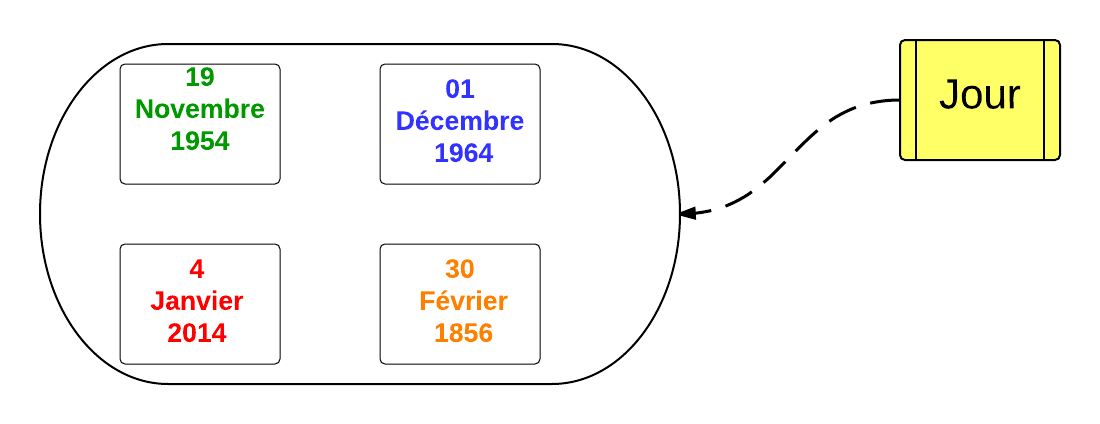
\includegraphics{Jour.png}}
\caption{Jour}\end{figure}

\textbf{Exemples}

Voici quelque exemples de classes.
\begin{itemize}
\item {} 
Point : pour définir un point dans le plan \(P(x,y)\).

\item {} 
Personne: définition d'une personne.

\item {} 
Voiture.

\end{itemize}

En uml on peut représenter ces classes, avec un diagramme de classes:
\begin{figure}[htbp]
\centering
\capstart

\scalebox{0.500000}{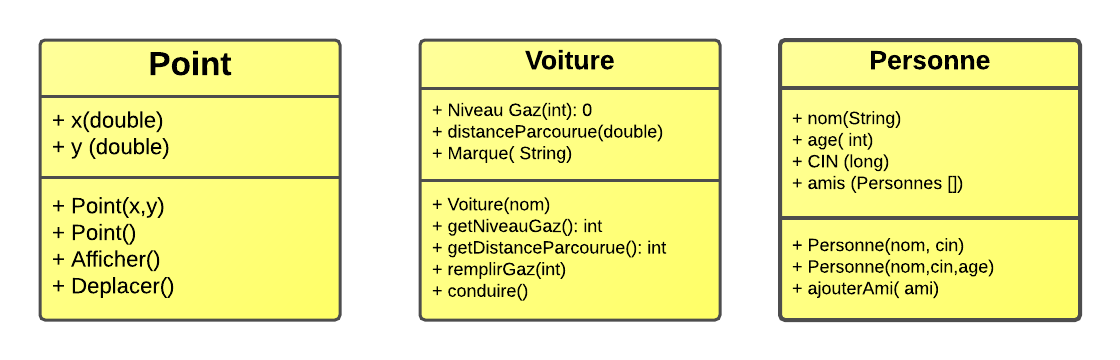
\includegraphics{classes1.png}}
\caption{Diagram des classes}\end{figure}


\subsection{Point}
\label{classes:point}
En se basant sur le diagramme \textbf{UML}, voici la définition de la classe Point

\begin{Verbatim}[commandchars=\\\{\},numbers=left,firstnumber=1,stepnumber=1]
\PYG{k+kd}{class} \PYG{n+nc}{Point}
\PYG{o}{\PYGZob{}}
    \PYG{c+c1}{//Attributs}
    \PYG{k+kd}{public} \PYG{k+kt}{double} \PYG{n}{x}\PYG{o}{;}
    \PYG{k+kd}{public} \PYG{k+kt}{double} \PYG{n}{y}\PYG{o}{;}


    \PYG{c+c1}{//Constructeurs}
    \PYG{k+kd}{public} \PYG{n+nf}{Point}\PYG{o}{(}\PYG{o}{)}
    \PYG{o}{\PYGZob{}}
        \PYG{k}{this}\PYG{o}{.}\PYG{n+na}{x}\PYG{o}{=}\PYG{l+m+mf}{0.0}\PYG{o}{;}
        \PYG{k}{this}\PYG{o}{.}\PYG{n+na}{y}\PYG{o}{=}\PYG{l+m+mf}{0.0}\PYG{o}{;}
    \PYG{o}{\PYGZcb{}}

    \PYG{k+kd}{public} \PYG{n+nf}{Point}\PYG{o}{(}\PYG{k+kt}{double} \PYG{n}{x}\PYG{o}{,}\PYG{k+kt}{double} \PYG{n}{y}\PYG{o}{)}
    \PYG{o}{\PYGZob{}}
        \PYG{k}{this}\PYG{o}{.}\PYG{n+na}{x}\PYG{o}{=}\PYG{n}{x}\PYG{o}{;}
        \PYG{k}{this}\PYG{o}{.}\PYG{n+na}{y}\PYG{o}{=}\PYG{n}{y}\PYG{o}{;}
    \PYG{o}{\PYGZcb{}}


    \PYG{c+c1}{//methode pour afficher le point}
    \PYG{k+kd}{public} \PYG{k+kt}{void} \PYG{n+nf}{afficher}\PYG{o}{(}\PYG{o}{)}
    \PYG{o}{\PYGZob{}}
        \PYG{n}{System}\PYG{o}{.}\PYG{n+na}{out}\PYG{o}{.}\PYG{n+na}{printf}\PYG{o}{(}\PYG{l+s}{\PYGZdq{}P(\PYGZpc{}.2f,\PYGZpc{}.2f)\PYGZbs{}n\PYGZdq{}}\PYG{o}{,}\PYG{k}{this}\PYG{o}{.}\PYG{n+na}{x}\PYG{o}{,}\PYG{k}{this}\PYG{o}{.}\PYG{n+na}{y}\PYG{o}{)}\PYG{o}{;}
    \PYG{o}{\PYGZcb{}}

    \PYG{k+kd}{public} \PYG{k+kt}{void} \PYG{n+nf}{deplacer}\PYG{o}{(}\PYG{k+kt}{double} \PYG{n}{dx}\PYG{o}{,}\PYG{k+kt}{double} \PYG{n}{dy}\PYG{o}{)}
    \PYG{o}{\PYGZob{}}
        \PYG{c+c1}{//fonction pour déplacer le point}
        \PYG{k}{this}\PYG{o}{.}\PYG{n+na}{x}\PYG{o}{+}\PYG{o}{=}\PYG{n}{dx}\PYG{o}{;}
        \PYG{k}{this}\PYG{o}{.}\PYG{n+na}{y}\PYG{o}{+}\PYG{o}{=}\PYG{n}{dy}\PYG{o}{;}
    \PYG{o}{\PYGZcb{}}


\PYG{o}{\PYGZcb{}}
\end{Verbatim}

Un programme qui va utiliser cette classe.

\begin{Verbatim}[commandchars=\\\{\},numbers=left,firstnumber=1,stepnumber=1]
\PYG{c+c1}{//codes/chap06/PointDriver.java}

\PYG{k+kd}{class} \PYG{n+nc}{PointDriver} \PYG{o}{\PYGZob{}}

    \PYG{k+kd}{public} \PYG{k+kd}{static} \PYG{k+kt}{void} \PYG{n+nf}{main}\PYG{o}{(}\PYG{n}{String}\PYG{o}{[}\PYG{o}{]} \PYG{n}{args}\PYG{o}{)} \PYG{o}{\PYGZob{}}

        \PYG{c+c1}{//Creation d\PYGZsq{}un object point}

        \PYG{n}{Point} \PYG{n}{A}\PYG{o}{=}\PYG{k}{new} \PYG{n}{Point}\PYG{o}{(}\PYG{l+m+mi}{2}\PYG{o}{,}\PYG{l+m+mi}{4}\PYG{o}{)}\PYG{o}{;}

        \PYG{c+c1}{//Afficher le point}
        \PYG{n}{System}\PYG{o}{.}\PYG{n+na}{out}\PYG{o}{.}\PYG{n+na}{println}\PYG{o}{(}\PYG{l+s}{\PYGZdq{}Les coordonées du points sont : \PYGZdq{}}\PYG{o}{)}\PYG{o}{;}
        \PYG{n}{A}\PYG{o}{.}\PYG{n+na}{afficher}\PYG{o}{(}\PYG{o}{)}\PYG{o}{;}

        \PYG{c+c1}{//Déplacer le point}
        \PYG{n}{A}\PYG{o}{.}\PYG{n+na}{deplacer}\PYG{o}{(}\PYG{l+m+mi}{1}\PYG{o}{,}\PYG{o}{\PYGZhy{}}\PYG{l+m+mi}{3}\PYG{o}{)}\PYG{o}{;}

        \PYG{c+c1}{//Afficher les nouvelles coordonnées du point}
        \PYG{n}{System}\PYG{o}{.}\PYG{n+na}{out}\PYG{o}{.}\PYG{n+na}{println}\PYG{o}{(}\PYG{l+s}{\PYGZdq{}Le nouveau point:\PYGZdq{}}\PYG{o}{)}\PYG{o}{;}
        \PYG{n}{A}\PYG{o}{.}\PYG{n+na}{afficher}\PYG{o}{(}\PYG{o}{)}\PYG{o}{;}
    \PYG{o}{\PYGZcb{}}

\PYG{o}{\PYGZcb{}}
\end{Verbatim}

\textbf{Question}
\begin{enumerate}
\item {} 
Ajouter une lettre comme nom du point.

\item {} 
Ajouter une méthode pour changer le nom du point.

\item {} 
Avec cette implémentation, est ce qu'un point connaît son \textbf{symétrique}.

\end{enumerate}
\begin{gather}
\begin{split}si A(x,y) \Longrightarrow S(-x,-y)\end{split}\notag
\end{gather}

\bigskip\hrule{}\bigskip



\subsection{Client Bancaire}
\label{classes:client-bancaire}
Construire en java une classe qui représente un client dans une banque.
\begin{figure}[htbp]
\centering
\capstart

\scalebox{0.700000}{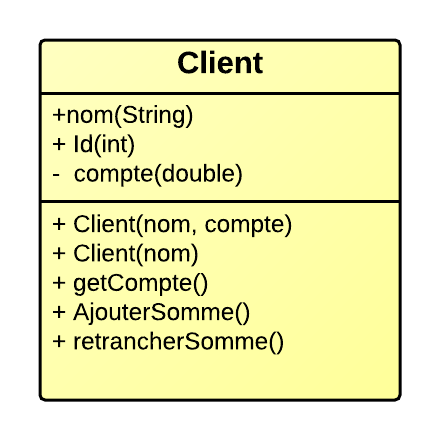
\includegraphics{Client.png}}
\caption{Client diagramme}\end{figure}

\begin{notice}{note}{Note:}\begin{itemize}
\item {} 
L'identifiant \textbf{id} du client doit vérifier :\(id \in [1,15]\). et \emph{ne peut pas} être modifié une foie un client est enregistré.

\item {} 
On doit pas accéder et changer au compte directement mais a travers une \textbf{interface} (API).

\item {} 
Dans le diagramme \emph{UML}, lister les fonctions qui indique cette \textbf{interface}.

\end{itemize}
\end{notice}

\begin{Verbatim}[commandchars=\\\{\},numbers=left,firstnumber=1,stepnumber=1]
\PYG{c+c1}{//codes/chap06/Client.java}

\PYG{c+cm}{/**}
\PYG{c+cm}{*   Class Client qui représente un client dans une banque}
\PYG{c+cm}{*/}
\PYG{k+kn}{import} \PYG{n+nn}{java.util.Random}\PYG{o}{;}

\PYG{k+kd}{class} \PYG{n+nc}{Client} \PYG{o}{\PYGZob{}}

    \PYG{c+cm}{/**}
\PYG{c+cm}{    * Attributs de la classe}
\PYG{c+cm}{    */}

    \PYG{k+kd}{private} \PYG{k+kt}{int} \PYG{n}{id}\PYG{o}{;}
    \PYG{k+kd}{private} \PYG{k+kt}{double} \PYG{n}{compte}\PYG{o}{;}
    \PYG{k+kd}{public} \PYG{n}{String} \PYG{n}{nom}\PYG{o}{;}


    \PYG{c+cm}{/**}
\PYG{c+cm}{    *  Constructeurs}
\PYG{c+cm}{    */}
    \PYG{n}{Client}\PYG{o}{(}\PYG{n}{String} \PYG{n}{nom}\PYG{o}{,}\PYG{k+kt}{double} \PYG{n}{compte}\PYG{o}{)}
    \PYG{o}{\PYGZob{}}
        \PYG{c+c1}{//constructeur avec un nom et compte}
    \PYG{o}{\PYGZcb{}}

    \PYG{n}{Client}\PYG{o}{(}\PYG{n}{String} \PYG{n}{nom}\PYG{o}{)}
    \PYG{o}{\PYGZob{}}
        \PYG{c+c1}{//Constructeur par un nom}
    \PYG{o}{\PYGZcb{}}

    \PYG{c+cm}{/**}
\PYG{c+cm}{    * Méthodes}
\PYG{c+cm}{    */}

    \PYG{c+c1}{//getter pour compte}
    \PYG{k+kt}{double} \PYG{n+nf}{getCompte}\PYG{o}{(}\PYG{o}{)}
    \PYG{o}{\PYGZob{}}
        \PYG{c+c1}{//code}
    \PYG{o}{\PYGZcb{}}


    \PYG{k+kt}{void} \PYG{n+nf}{ajouterSomme}\PYG{o}{(}\PYG{k+kt}{double} \PYG{n}{ajout}\PYG{o}{)}
    \PYG{o}{\PYGZob{}}
       \PYG{c+c1}{//code}
    \PYG{o}{\PYGZcb{}}

    \PYG{k+kt}{void} \PYG{n+nf}{retrancherSomme}\PYG{o}{(}\PYG{k+kt}{double} \PYG{n}{retrait}\PYG{o}{)}
    \PYG{o}{\PYGZob{}}
        \PYG{c+c1}{//code}
    \PYG{o}{\PYGZcb{}}

    \PYG{k+kt}{void} \PYG{n+nf}{afficher}\PYG{o}{(}\PYG{o}{)}
    \PYG{o}{\PYGZob{}}
        \PYG{c+c1}{//code}
    \PYG{o}{\PYGZcb{}}
\PYG{o}{\PYGZcb{}}
\end{Verbatim}

Programme utilisant cette classe.

\begin{Verbatim}[commandchars=\\\{\},numbers=left,firstnumber=1,stepnumber=1]
\PYG{c+c1}{//codes/chap06/ClientDriver.java}


\PYG{k+kd}{class} \PYG{n+nc}{ClientDriver} \PYG{o}{\PYGZob{}}

    \PYG{k+kd}{public} \PYG{k+kd}{static} \PYG{k+kt}{void} \PYG{n+nf}{main}\PYG{o}{(}\PYG{n}{String}\PYG{o}{[}\PYG{o}{]} \PYG{n}{args}\PYG{o}{)} \PYG{o}{\PYGZob{}}

        \PYG{c+c1}{//Construire un client simple client}
        \PYG{n}{Client} \PYG{n}{cl1}\PYG{o}{=}\PYG{k}{new} \PYG{n}{Client}\PYG{o}{(}\PYG{l+s}{\PYGZdq{}MTI\PYGZdq{}}\PYG{o}{,}\PYG{l+m+mi}{4000}\PYG{o}{)}\PYG{o}{;}
        \PYG{n}{cl1}\PYG{o}{.}\PYG{n+na}{afficher}\PYG{o}{(}\PYG{o}{)}\PYG{o}{;}

        \PYG{c+c1}{//Changer le compte manuellement donnera une erreur}
        \PYG{c+c1}{//cl1.compte=cl1.compte+1000;}

        \PYG{c+c1}{//la bonne méthode est d\PYGZsq{}utiliser le mutateur}
        \PYG{n}{cl1}\PYG{o}{.}\PYG{n+na}{ajouterSomme}\PYG{o}{(}\PYG{l+m+mi}{1000}\PYG{o}{)}\PYG{o}{;}
        \PYG{n}{cl1}\PYG{o}{.}\PYG{n+na}{afficher}\PYG{o}{(}\PYG{o}{)}\PYG{o}{;}
    \PYG{o}{\PYGZcb{}}
\PYG{o}{\PYGZcb{}}
\end{Verbatim}

\begin{notice}{warning}{Warning:}
La ligne 13 du programme essaie de modifier un attribut \textbf{privé}, ce qui va générer une erreur.
\end{notice}


\subsection{Attributs statiques}
\label{classes:attributs-statiques}
Chaque Objet d'une classe possède sa propre \textbf{copie} des attributs de la classes. mais dans certains cas, juste une \textbf{seule copie} de la classe pourra être \emph{partagée} entre tous objets.

Un attribut \textbf{statique}, ou \emph{attribut de la classe} est utilisé dans ces cas. pour stocker une information générale de la classe et sera partagé par tous les \textbf{instances} de cette classe.

La déclaration de type de membre est réalisé par le mot clé \textbf{static}.


\subsubsection{Exemples}
\label{classes:exemples}
Quelque exemples des membres statiques.
\begin{itemize}
\item {} 
Nombre de Clients dans une banque.

\item {} 
Type de stockage d'une structure de donnée.

\item {} 
Type d'orientation des formes géométriques.

\end{itemize}

\begin{Verbatim}[commandchars=\\\{\}]
\PYG{k+kd}{class} \PYG{n+nc}{Client}
\PYG{o}{\PYGZob{}}
    \PYG{k+kd}{private} \PYG{k+kd}{static} \PYG{n}{nb\PYGZus{}Clients}\PYG{o}{=}\PYG{l+m+mf}{0.0}\PYG{o}{;}
    \PYG{k+kd}{private} \PYG{n}{String} \PYG{n}{nom}
    \PYG{k+kd}{private} \PYG{k+kt}{double} \PYG{n}{compte}\PYG{o}{;}
\PYG{o}{\PYGZcb{}}
\end{Verbatim}


\subsubsection{Exemple illustratif}
\label{classes:exemple-illustratif}
Dans cet exemple on se propose de créer un modèle simple d'une classe \textbf{Guerrier}.
\begin{figure}[htbp]
\centering
\capstart

\scalebox{0.600000}{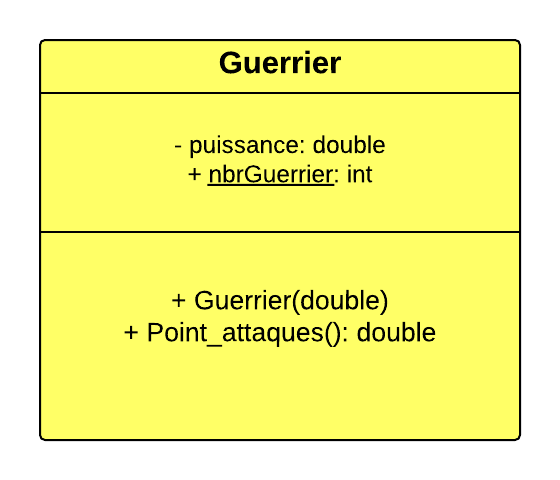
\includegraphics{guerrier1.png}}
\caption{Diagramme de la classe Guerrier. (les membres statiques sont en italiques)}\end{figure}

\begin{notice}{note}{Note:}
Pour calculer les points d'attaques d'un guerrier en utilise la formule suivante:

\begin{Verbatim}[commandchars=\\\{\}]
Ps\PYGZus{}attaques=(puissance*1000)+300*nbrGuerrier.
\end{Verbatim}
\end{notice}

\begin{center}Exercice
\end{center}\begin{enumerate}
\item {} 
Ajouter une méthode pour afficher le nombre de guerrier?

\item {} 
Que remarquez vous?

\end{enumerate}


\subsubsection{Classe math}
\label{classes:classe-math}
La classe \textbf{math} utilise la notion de
\begin{itemize}
\item {} 
membre statique

\item {} 
fonctions statiques

\end{itemize}

Pour fournir une implémentation pour la plupart des  \textbf{constantes} et \textbf{fonctions} mathématiques usuelles.

\begin{Verbatim}[commandchars=\\\{\},numbers=left,firstnumber=1,stepnumber=1]
\PYG{k+kd}{public} \PYG{k+kd}{class} \PYG{n+nc}{MathExemples} \PYG{o}{\PYGZob{}}

    \PYG{k+kd}{public} \PYG{k+kd}{static} \PYG{k+kt}{void} \PYG{n+nf}{main}\PYG{o}{(}\PYG{n}{String}\PYG{o}{[}\PYG{o}{]} \PYG{n}{args}\PYG{o}{)} \PYG{o}{\PYGZob{}}

        \PYG{c+c1}{//Afficher la valeur de pi}
        \PYG{n}{System}\PYG{o}{.}\PYG{n+na}{out}\PYG{o}{.}\PYG{n+na}{println}\PYG{o}{(}\PYG{l+s}{\PYGZdq{}valeur de pi= \PYGZdq{}}\PYG{o}{+}\PYG{n}{Math}\PYG{o}{.}\PYG{n+na}{PI}\PYG{o}{)}\PYG{o}{;}

        \PYG{c+c1}{//Afficher la valeur de e}
        \PYG{n}{System}\PYG{o}{.}\PYG{n+na}{out}\PYG{o}{.}\PYG{n+na}{println}\PYG{o}{(}\PYG{l+s}{\PYGZdq{}valeur de e= \PYGZdq{}}\PYG{o}{+}\PYG{n}{Math}\PYG{o}{.}\PYG{n+na}{E}\PYG{o}{)}\PYG{o}{;}


        \PYG{c+c1}{//Quelque fonctions usuels}
        \PYG{k+kt}{double} \PYG{n}{pi}\PYG{o}{=}\PYG{n}{Math}\PYG{o}{.}\PYG{n+na}{PI}\PYG{o}{;}
        \PYG{n}{System}\PYG{o}{.}\PYG{n+na}{out}\PYG{o}{.}\PYG{n+na}{println}\PYG{o}{(}\PYG{l+s}{\PYGZdq{}cos(3pi/2)= \PYGZdq{}}\PYG{o}{+}\PYG{n}{Math}\PYG{o}{.}\PYG{n+na}{cos}\PYG{o}{(}\PYG{l+m+mi}{3}\PYG{o}{*}\PYG{n}{pi}\PYG{o}{/}\PYG{l+m+mf}{2.0}\PYG{o}{)}\PYG{o}{)}\PYG{o}{;}
        \PYG{n}{System}\PYG{o}{.}\PYG{n+na}{out}\PYG{o}{.}\PYG{n+na}{println}\PYG{o}{(}\PYG{l+s}{\PYGZdq{}sin(3pi/2= \PYGZdq{}}\PYG{o}{+}\PYG{n}{Math}\PYG{o}{.}\PYG{n+na}{sin}\PYG{o}{(}\PYG{l+m+mi}{3}\PYG{o}{*}\PYG{n}{pi}\PYG{o}{/}\PYG{l+m+mf}{2.0}\PYG{o}{)}\PYG{o}{)}\PYG{o}{;}

        \PYG{c+c1}{//fonction logarithmes}
        \PYG{n}{System}\PYG{o}{.}\PYG{n+na}{out}\PYG{o}{.}\PYG{n+na}{println}\PYG{o}{(}\PYG{l+s}{\PYGZdq{}Log(430)=\PYGZdq{}}\PYG{o}{+}\PYG{n}{Math}\PYG{o}{.}\PYG{n+na}{log}\PYG{o}{(}\PYG{l+m+mi}{430}\PYG{o}{)}\PYG{o}{)}\PYG{o}{;}


        \PYG{c+c1}{//fonction exponentielle}
        \PYG{n}{System}\PYG{o}{.}\PYG{n+na}{out}\PYG{o}{.}\PYG{n+na}{println}\PYG{o}{(}\PYG{l+s}{\PYGZdq{}exp(\PYGZhy{}500)= \PYGZdq{}}\PYG{o}{+}\PYG{n}{Math}\PYG{o}{.}\PYG{n+na}{exp}\PYG{o}{(}\PYG{o}{\PYGZhy{}}\PYG{l+m+mi}{500}\PYG{o}{)}\PYG{o}{)}\PYG{o}{;}

    \PYG{o}{\PYGZcb{}}

\PYG{o}{\PYGZcb{}}
\end{Verbatim}


\subsection{Union\_Find}
\label{classes:union-find}

\section{Relations entre classes}
\label{classes2:relations-entre-classes}\label{classes2::doc}
On peut construire des classes complexes, qui peuvent contenir d'autre classes, ou améliore  ou modifie le comportement des classes existantes.


\subsection{Composition}
\label{classes2:composition}
Un lien de \textbf{composition} (fait partie) symbolise l'existence d'une relation particulière, dite `forte', entre deux entités (classes). par exemple:
\begin{itemize}
\item {} 
Un \textbf{Segment} contient deux \emph{points}.

\item {} 
Une \textbf{Voiture} doit contenir un \emph{Carburateur}.

\item {} 
Une \textbf{Ordinateur} ne peut pas fonctionner sans une \emph{carte mère}.

\end{itemize}

Donc une \textbf{composition} est définie par les points suivants:

\begin{notice}{note}{Note:}
Par exemple dans le premier exemple, on dit que la classe \emph{Point} est \textbf{agrégée} à la classe \emph{Segment}.
\end{notice}
\begin{itemize}
\item {} \begin{description}
\item[{Durée de vie:}] \leavevmode
Toute classe agrégée est détruite quand sa classe \emph{composite}  est détruite.

\end{description}

\item {} \begin{description}
\item[{Exclusivité:}] \leavevmode
Une classe agrégée ne peut exister que pour une seule classe composite.

\end{description}

\end{itemize}


\subsubsection{exemples:}
\label{classes2:exemples}
\begin{Verbatim}[commandchars=\\\{\}]
\PYG{k+kd}{public} \PYG{k+kd}{class} \PYG{n+nc}{Voiture}
\PYG{o}{\PYGZob{}}
    \PYG{c+c1}{//Voiture est responsable de l\PYGZsq{}objet carb.}
    \PYG{k+kd}{private} \PYG{n}{Carburateur} \PYG{n}{carb}\PYG{o}{;}

    \PYG{k+kd}{public} \PYG{n+nf}{Voiture}\PYG{o}{(}\PYG{o}{.}\PYG{o}{.}\PYG{o}{.}\PYG{o}{)}
    \PYG{o}{\PYGZob{}}
       \PYG{c+c1}{//le constructeur Voiture doit aussi construire carb}
       \PYG{n}{carb}\PYG{o}{=}\PYG{k}{new} \PYG{n}{Carburateur}\PYG{o}{(}\PYG{o}{.}\PYG{o}{.}\PYG{o}{.}\PYG{o}{)}
    \PYG{o}{\PYGZcb{}}

\PYG{o}{\PYGZcb{}}
\end{Verbatim}


\paragraph{Exercice:}
\label{classes2:exercice}\begin{enumerate}
\item {} 
Créer une classe \textbf{Segment} en utilisant la classe prédéfinie \textbf{Point}.

\end{enumerate}


\subsection{Agrégation}
\label{classes2:agregation}
l'agrégation permet de définir une entité comme étant liée à \textbf{plusieurs} entités de classe différentes. C'est une généralisation de la composition, qui \textbf{n'entraîne} pas l'appartenance par exemple:
\begin{itemize}
\item {} 
Une faculté utilise un ensemble de \textbf{Professeurs}.

\item {} 
Un aéroport agrège plusieurs \textbf{avions}.

\end{itemize}

\begin{Verbatim}[commandchars=\\\{\}]
\PYG{k+kd}{public} \PYG{k+kd}{class} \PYG{n+nc}{Faculte}
\PYG{o}{\PYGZob{}}
   \PYG{c+c1}{// liste des professeurs}
   \PYG{k+kd}{private} \PYG{n}{Professeur}\PYG{o}{[}\PYG{o}{]} \PYG{n}{profs}\PYG{o}{;}

   \PYG{k+kd}{public} \PYG{n+nf}{Faculte}\PYG{o}{(}\PYG{o}{.}\PYG{o}{.}\PYG{o}{.}\PYG{o}{)}
   \PYG{o}{\PYGZob{}}
          \PYG{c+c1}{//la classe faculté n\PYGZsq{}est pas responsable}
          \PYG{c+c1}{//pour la création des professeurs. il les ajoutes}
   \PYG{o}{\PYGZcb{}}
\PYG{o}{\PYGZcb{}}
\end{Verbatim}
\begin{enumerate}
\item {} 
Ecrire un code en java pour le modèle suivant:

\end{enumerate}
\begin{figure}[htbp]
\centering
\capstart

\scalebox{0.600000}{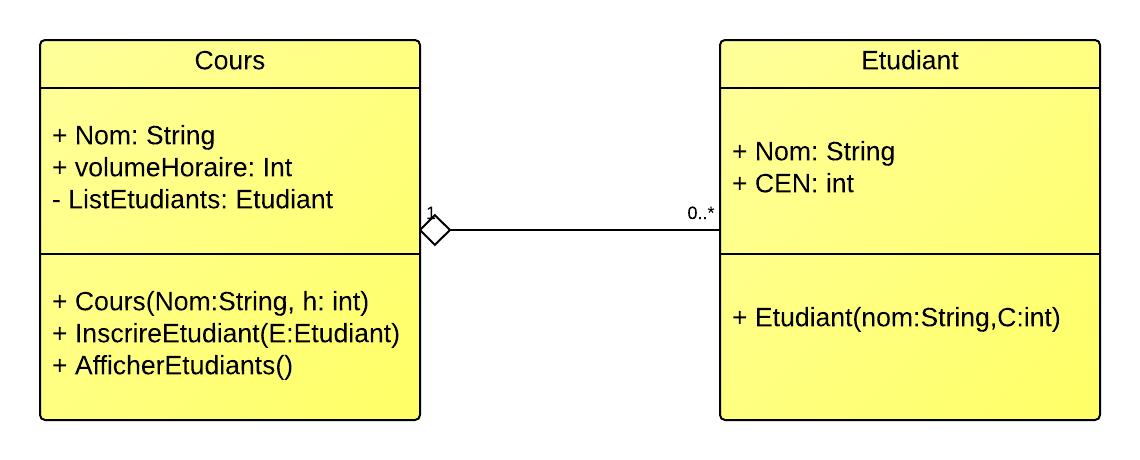
\includegraphics{agregation.png}}
\caption{Diagramme d'agrégation.}\end{figure}


\subsection{Héritage}
\label{classes2:heritage}
Le concept d'héritage est un des concepts les plus important dans la programmation orienté objet. C'est un mécanisme permettant de créer une nouvelle classe \textbf{à partir} d'une classe existante en lui proférant ses propriétés et ses méthodes.

Ainsi, pour définir une nouvelle classe, il suffit de la faire hériter d'une classe existante et de lui ajouter de nouvelles propriétés/méthodes.

Par un exemple un \emph{Lion} peut être modélisé comme un \textbf{carnivore} en lui ajoutant les d'autre propriétés.

\begin{notice}{note}{Note:}
Dans l'exemple précédant on dit que la classe \textbf{Lion} est dit classe \emph{mère} de la classe \textbf{Lion}.
\end{notice}
\begin{figure}[htbp]
\centering
\capstart

\scalebox{0.700000}{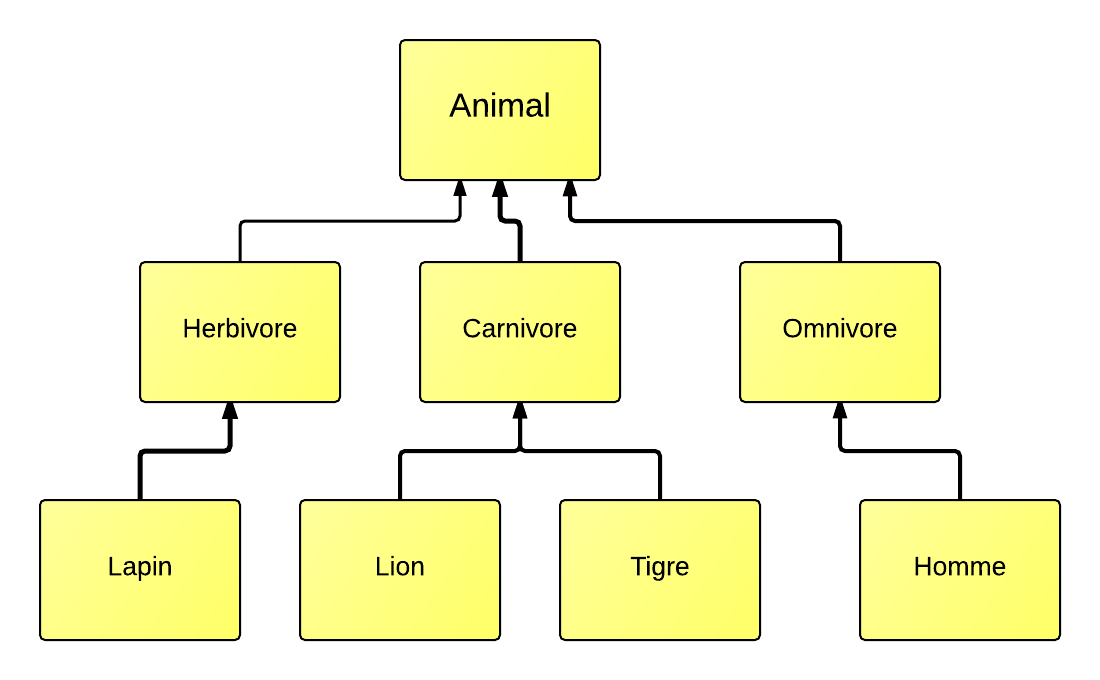
\includegraphics{heritage.png}}
\caption{Diagramme d'héritage}\end{figure}

En java pour indiquer qu'une classe B hérite d'une classe A, on utilise le mot clé \textbf{extends} dans la déclaration de la classe.

\begin{Verbatim}[commandchars=\\\{\}]
\PYG{k+kd}{public} \PYG{k+kd}{class} \PYG{n+nc}{B} \PYG{k+kd}{extends} \PYG{n}{A}
\PYG{o}{\PYGZob{}}
      \PYG{o}{.}\PYG{o}{.}\PYG{o}{.}
\PYG{o}{\PYGZcb{}}
\end{Verbatim}

Dans cette section on propose un exemple simple pour bien assimiler syntaxe concernant l'héritage. Le but de l'exemple est de créer une classe \textbf{Point Coloré} en héritant de la classe \textbf{Point} et en utilisant une composition avec la classe \textbf{Color}.

\begin{Verbatim}[commandchars=\\\{\},numbers=left,firstnumber=1,stepnumber=1]
\PYG{k+kd}{public} \PYG{k+kd}{class} \PYG{n+nc}{Point} \PYG{o}{\PYGZob{}}
	
	\PYG{k+kd}{protected} \PYG{k+kt}{double} \PYG{n}{x}\PYG{o}{;}
	\PYG{k+kd}{protected} \PYG{k+kt}{double} \PYG{n}{y}\PYG{o}{;}
	\PYG{k+kd}{protected} \PYG{k+kt}{char} \PYG{n}{nom}\PYG{o}{;}
	
	\PYG{k+kd}{public} \PYG{n+nf}{Point}\PYG{o}{(}\PYG{o}{)}
	\PYG{o}{\PYGZob{}}
		\PYG{k}{this}\PYG{o}{.}\PYG{n+na}{x}\PYG{o}{=}\PYG{l+m+mi}{0}\PYG{o}{;}
		\PYG{k}{this}\PYG{o}{.}\PYG{n+na}{y}\PYG{o}{=}\PYG{l+m+mi}{0}\PYG{o}{;}
		\PYG{k}{this}\PYG{o}{.}\PYG{n+na}{nom}\PYG{o}{=}\PYG{l+s+sc}{\PYGZsq{}O\PYGZsq{}}\PYG{o}{;}
	\PYG{o}{\PYGZcb{}}
	
	\PYG{k+kd}{public} \PYG{n+nf}{Point}\PYG{o}{(}\PYG{k+kt}{double} \PYG{n}{x}\PYG{o}{,}\PYG{k+kt}{double} \PYG{n}{y}\PYG{o}{,}\PYG{k+kt}{char} \PYG{n}{N}\PYG{o}{)}
	\PYG{o}{\PYGZob{}}
		\PYG{k}{this}\PYG{o}{.}\PYG{n+na}{x}\PYG{o}{=}\PYG{n}{x}\PYG{o}{;}
		\PYG{k}{this}\PYG{o}{.}\PYG{n+na}{y}\PYG{o}{=}\PYG{n}{y}\PYG{o}{;}
		\PYG{k}{this}\PYG{o}{.}\PYG{n+na}{nom}\PYG{o}{=}\PYG{n}{N}\PYG{o}{;}
	\PYG{o}{\PYGZcb{}}
	
	\PYG{k+kd}{public} \PYG{k+kt}{void} \PYG{n+nf}{afficher}\PYG{o}{(}\PYG{o}{)}
	\PYG{o}{\PYGZob{}}
		\PYG{n}{System}\PYG{o}{.}\PYG{n+na}{out}\PYG{o}{.}\PYG{n+na}{printf}\PYG{o}{(}\PYG{l+s}{\PYGZdq{}\PYGZpc{}c=(\PYGZpc{}.2f,\PYGZpc{}.2f)\PYGZbs{}n\PYGZdq{}}\PYG{o}{,}\PYG{n}{nom}\PYG{o}{,}\PYG{n}{x}\PYG{o}{,}\PYG{n}{y}\PYG{o}{)}\PYG{o}{;}
	\PYG{o}{\PYGZcb{}}
	
	\PYG{k+kd}{public} \PYG{k+kt}{void} \PYG{n+nf}{deplacer}\PYG{o}{(}\PYG{k+kt}{double} \PYG{n}{dx}\PYG{o}{,}\PYG{k+kt}{double} \PYG{n}{dy}\PYG{o}{)}
	\PYG{o}{\PYGZob{}}
		\PYG{n}{x}\PYG{o}{+}\PYG{o}{=}\PYG{n}{dx}\PYG{o}{;}
		\PYG{n}{y}\PYG{o}{+}\PYG{o}{=}\PYG{n}{dy}\PYG{o}{;}
	\PYG{o}{\PYGZcb{}}

\PYG{o}{\PYGZcb{}}
\end{Verbatim}

\begin{Verbatim}[commandchars=\\\{\},numbers=left,firstnumber=1,stepnumber=1]
\PYG{k+kn}{import} \PYG{n+nn}{java.awt.Color}\PYG{o}{;}

\PYG{c+c1}{//class héritant de Point}
\PYG{k+kd}{public} \PYG{k+kd}{class} \PYG{n+nc}{PointColor} \PYG{k+kd}{extends} \PYG{n}{Point} \PYG{o}{\PYGZob{}}
	
	\PYG{c+c1}{//ajout d\PYGZsq{}un attribut couleur}
	\PYG{k+kd}{private} \PYG{n}{Color} \PYG{n}{c}\PYG{o}{;}
	
	\PYG{c+c1}{//Constructeur par defaut}
	\PYG{k+kd}{public} \PYG{n+nf}{PointColor}\PYG{o}{(}\PYG{o}{)}
	\PYG{o}{\PYGZob{}}
		\PYG{c+c1}{//appeler le constructeur par defaut de Point}
		\PYG{k+kd}{super}\PYG{o}{(}\PYG{o}{)}\PYG{o}{;}
		
		\PYG{c+c1}{//ajouter une couleur blanche}
		\PYG{n}{c}\PYG{o}{=}\PYG{k}{new} \PYG{n}{Color}\PYG{o}{(}\PYG{l+m+mi}{255}\PYG{o}{,} \PYG{l+m+mi}{255}\PYG{o}{,} \PYG{l+m+mi}{255}\PYG{o}{)}\PYG{o}{;}
	\PYG{o}{\PYGZcb{}}
	
	\PYG{k+kd}{public} \PYG{n+nf}{PointColor}\PYG{o}{(}\PYG{k+kt}{double} \PYG{n}{x}\PYG{o}{,}\PYG{k+kt}{double} \PYG{n}{y}\PYG{o}{,}\PYG{k+kt}{char} \PYG{n}{N}\PYG{o}{,}\PYG{n}{Color} \PYG{n}{C}\PYG{o}{)}
	\PYG{o}{\PYGZob{}}
		\PYG{c+c1}{//appeler le constructeur de Point}
		\PYG{k+kd}{super}\PYG{o}{(}\PYG{n}{x}\PYG{o}{,}\PYG{n}{y}\PYG{o}{,}\PYG{n}{N}\PYG{o}{)}\PYG{o}{;}
		
		\PYG{c+c1}{//affecter la couleur}
		\PYG{k}{this}\PYG{o}{.}\PYG{n+na}{c}\PYG{o}{=}\PYG{n}{C}\PYG{o}{;}
	\PYG{o}{\PYGZcb{}}
	
	\PYG{c+c1}{//Afficher le point en utilisant la fonction de Point}
	\PYG{k+kd}{public} \PYG{k+kt}{void} \PYG{n+nf}{afficher}\PYG{o}{(}\PYG{o}{)}
	\PYG{o}{\PYGZob{}}
		\PYG{k+kd}{super}\PYG{o}{.}\PYG{n+na}{afficher}\PYG{o}{(}\PYG{o}{)}\PYG{o}{;}
		
		\PYG{c+c1}{//Afficher la partie manquante}
		\PYG{n}{System}\PYG{o}{.}\PYG{n+na}{out}\PYG{o}{.}\PYG{n+na}{println}\PYG{o}{(}\PYG{l+s}{\PYGZdq{}Couleur est \PYGZdq{}}\PYG{o}{+}\PYG{n}{c}\PYG{o}{)}\PYG{o}{;}
	\PYG{o}{\PYGZcb{}}
	
	\PYG{k+kd}{public} \PYG{k+kt}{void} \PYG{n+nf}{changerCouleur}\PYG{o}{(}\PYG{n}{Color} \PYG{n}{c}\PYG{o}{)}
	\PYG{o}{\PYGZob{}}
		\PYG{k}{this}\PYG{o}{.}\PYG{n+na}{c}\PYG{o}{=}\PYG{n}{c}\PYG{o}{;}
	\PYG{o}{\PYGZcb{}}
\PYG{o}{\PYGZcb{}}
\end{Verbatim}


\subsection{Surcharge}
\label{classes2:surcharge}

\subsection{Le mot clé final}
\label{classes2:le-mot-cle-final}
Le mot clé \textbf{final} doit être utilisé pour fixer l'état soit:
\begin{itemize}
\item {} 
Variable

\item {} 
Méthode

\item {} 
Classe

\end{itemize}


\subsubsection{Variables}
\label{classes2:variables}
Ajouté à une variable, ne permet plus de changer sa valeur.

\begin{Verbatim}[commandchars=\\\{\},numbers=left,firstnumber=1,stepnumber=1]
\PYG{k+kd}{public} \PYG{k+kd}{class} \PYG{n+nc}{FinalVariable} \PYG{o}{\PYGZob{}}
	
	\PYG{c+c1}{//variable final non modifiable}
	\PYG{k+kd}{final} \PYG{k+kd}{static} \PYG{k+kt}{double} \PYG{n}{g}\PYG{o}{=}\PYG{l+m+mf}{9.8}\PYG{o}{;} 
	
	\PYG{k+kd}{public} \PYG{k+kd}{static} \PYG{k+kt}{void} \PYG{n+nf}{main}\PYG{o}{(}\PYG{n}{String}\PYG{o}{[}\PYG{o}{]} \PYG{n}{args}\PYG{o}{)} \PYG{o}{\PYGZob{}}
		
		\PYG{c+c1}{//Afficher la valeur de g}
		\PYG{n}{System}\PYG{o}{.}\PYG{n+na}{out}\PYG{o}{.}\PYG{n+na}{println}\PYG{o}{(}\PYG{l+s}{\PYGZdq{}g= \PYGZdq{}}\PYG{o}{+}\PYG{n}{g}\PYG{o}{)}\PYG{o}{;}
		
		\PYG{c+c1}{//Changer la valeur de g donnera une erreur}
		\PYG{n}{g}\PYG{o}{+}\PYG{o}{=}\PYG{l+m+mi}{3}\PYG{o}{;}
	\PYG{o}{\PYGZcb{}}

\PYG{o}{\PYGZcb{}}
\end{Verbatim}


\subsubsection{Méthodes}
\label{classes2:methodes}
Pour une fonction, le mot \emph{final} indique qu'on peut plus la \textbf{surcharger}.

\begin{Verbatim}[commandchars=\\\{\},numbers=left,firstnumber=1,stepnumber=1]
\PYG{c+c1}{//une simple classe pour démontrer l\PYGZsq{}héritage}
\PYG{k+kd}{public} \PYG{k+kd}{class} \PYG{n+nc}{A} \PYG{o}{\PYGZob{}}
	
	\PYG{k+kd}{protected} \PYG{k+kt}{double} \PYG{n}{a}\PYG{o}{;}
	
	\PYG{c+c1}{//Constructeur simple}
	\PYG{k+kd}{public} \PYG{n+nf}{A}\PYG{o}{(}\PYG{k+kt}{double} \PYG{n}{a}\PYG{o}{)}
	\PYG{o}{\PYGZob{}}
		\PYG{k}{this}\PYG{o}{.}\PYG{n+na}{a}\PYG{o}{=}\PYG{n}{a}\PYG{o}{;}
	\PYG{o}{\PYGZcb{}}
	
	\PYG{c+c1}{//méthode simple pour afficher a}
	\PYG{k+kd}{public} \PYG{k+kt}{void} \PYG{n+nf}{method1}\PYG{o}{(}\PYG{o}{)}
	\PYG{o}{\PYGZob{}}
		\PYG{n}{System}\PYG{o}{.}\PYG{n+na}{out}\PYG{o}{.}\PYG{n+na}{println}\PYG{o}{(}\PYG{l+s}{\PYGZdq{}valeur de a= \PYGZdq{}}\PYG{o}{+}\PYG{n}{a}\PYG{o}{)}\PYG{o}{;}
	\PYG{o}{\PYGZcb{}}
	
	\PYG{c+c1}{//deuxième méthode non surchable pour afficher un message}
	\PYG{k+kd}{public} \PYG{k+kd}{final} \PYG{k+kt}{void} \PYG{n+nf}{method2}\PYG{o}{(}\PYG{o}{)}
	\PYG{o}{\PYGZob{}}
		\PYG{n}{System}\PYG{o}{.}\PYG{n+na}{out}\PYG{o}{.}\PYG{n+na}{println}\PYG{o}{(}\PYG{l+s}{\PYGZdq{}Message dans la classe A\PYGZdq{}}\PYG{o}{)}\PYG{o}{;}
	\PYG{o}{\PYGZcb{}}

\PYG{o}{\PYGZcb{}}
\end{Verbatim}

\begin{Verbatim}[commandchars=\\\{\},numbers=left,firstnumber=1,stepnumber=1]
\PYG{k+kd}{public} \PYG{k+kd}{class} \PYG{n+nc}{B} \PYG{k+kd}{extends} \PYG{n}{A} \PYG{o}{\PYGZob{}}
	
	\PYG{k+kd}{protected} \PYG{k+kt}{double} \PYG{n}{b}\PYG{o}{;}
	
	
	\PYG{k+kd}{public} \PYG{n+nf}{B}\PYG{o}{(}\PYG{k+kt}{double} \PYG{n}{a}\PYG{o}{,}\PYG{k+kt}{double} \PYG{n}{b}\PYG{o}{)}
	\PYG{o}{\PYGZob{}}	
		\PYG{k+kd}{super}\PYG{o}{(}\PYG{n}{a}\PYG{o}{)}\PYG{o}{;}
		\PYG{k}{this}\PYG{o}{.}\PYG{n+na}{b}\PYG{o}{=}\PYG{n}{b}\PYG{o}{;}
	\PYG{o}{\PYGZcb{}}
	
	\PYG{c+c1}{//surchage de la première méthode (possible}
	\PYG{k+kd}{public} \PYG{k+kt}{void} \PYG{n+nf}{method1}\PYG{o}{(}\PYG{o}{)}
	\PYG{o}{\PYGZob{}}
		\PYG{c+c1}{//appeler la méthode de la classe mère}
		\PYG{k+kd}{super}\PYG{o}{.}\PYG{n+na}{method1}\PYG{o}{(}\PYG{o}{)}\PYG{o}{;}
		
		\PYG{n}{System}\PYG{o}{.}\PYG{n+na}{out}\PYG{o}{.}\PYG{n+na}{println}\PYG{o}{(}\PYG{l+s}{\PYGZdq{}valeur de b= \PYGZdq{}}\PYG{o}{+}\PYG{n}{b}\PYG{o}{)}\PYG{o}{;}
	\PYG{o}{\PYGZcb{}}
	
	\PYG{c+c1}{//Ceci donnera une erreur car method2 est finale dans B}
	\PYG{c+c1}{//public void method2();}
	
	\PYG{k+kd}{public} \PYG{k+kd}{static} \PYG{k+kt}{void} \PYG{n+nf}{main}\PYG{o}{(}\PYG{n}{String} \PYG{o}{[}\PYG{o}{]}\PYG{n}{args}\PYG{o}{)}
	\PYG{o}{\PYGZob{}}
		\PYG{n}{B} \PYG{n}{var}\PYG{o}{=}\PYG{k}{new} \PYG{n}{B}\PYG{o}{(}\PYG{l+m+mi}{3}\PYG{o}{,}\PYG{l+m+mi}{2}\PYG{o}{)}\PYG{o}{;}
		
		\PYG{n}{var}\PYG{o}{.}\PYG{n+na}{method1}\PYG{o}{(}\PYG{o}{)}\PYG{o}{;}
		\PYG{n}{var}\PYG{o}{.}\PYG{n+na}{method2}\PYG{o}{(}\PYG{o}{)}\PYG{o}{;}
		
	\PYG{o}{\PYGZcb{}}
\PYG{o}{\PYGZcb{}}
\end{Verbatim}


\subsubsection{Classes}
\label{classes2:classes}
\begin{notice}{note}{Note:}
Ajouter l'attribut \emph{final} à une classe, indiquera que cette classe ne peut plus servir comme classe \textbf{mère} à une autre classe. (ie) \textbf{hériter} de cette classe est impossible.
\end{notice}


\chapter{Indices et tables}
\label{index:indices-et-tables}\begin{itemize}
\item {} 
\emph{genindex}

\item {} 
\emph{modindex}

\item {} 
\emph{search}

\end{itemize}



\renewcommand{\indexname}{Index}
\printindex
\end{document}
